\documentclass[11pt]{report}
\usepackage{graphicx}
\usepackage[margin = 2.5cm]{geometry}
\usepackage[T1]{fontenc}
\usepackage{setspace}
\usepackage{tikz}
\usepackage{amsmath}
\usepackage{amssymb}
\usepackage{verbatim}
\usepackage{lscape}

% checkmarks
\def\checkmark{\tikz\fill[scale=0.4](0,.35) -- (.25,0) -- (1,.7) -- (.25,.15) -- cycle;} 

% fancy chapter headers
\usepackage{titlesec, blindtext, color}
\definecolor{gray75}{gray}{0.75}
\newcommand{\hsp}{\hspace{20pt}}
\titleformat{\chapter}[hang]{\Huge\bfseries}{\thechapter\hsp\textcolor{gray75}{|}\hsp}{0pt}{\Huge\bfseries}

% captions
\usepackage[labelfont=bf]{caption}
\captionsetup{skip=7pt, font=footnotesize} %,font={stretch=1}

% tables
\usepackage{multirow}
%\usepackage{longtable} 
\usepackage{array}
%\usepackage{verbatim} 
\usepackage{csvsimple}

% clinkable links 
\usepackage[hidelinks]{hyperref}
\hypersetup{
    colorlinks=false, %set true if you want colored links
    linktoc=all     %set to all if you want both sections and subsections linked
    %linkcolor=blue,  %choose some color if you want links to stand out
}

% Bibliography
\usepackage[backend=bibtex, natbib=true, url=false, doi=true, isbn=false, style=authoryear-comp, eprint=false, maxbibnames= 20, firstinits=true, maxcitenames=2]{biblatex}
\addbibresource{library2.bib}
% remove "" around title
\DeclareFieldFormat
  [article,inbook,incollection,inproceedings,patent,thesis,unpublished]
  {title}{#1\isdot}
% author: last name, first name
\DeclareNameAlias{sortname}{last-first}
% remove pp before pages
\DeclareFieldFormat{pages}{#1}
% remove comma / space before pages, and put colon instead
%\renewcommand*{\bibpagespunct}{%
%\ifentrytype{article}
%  {\addcolon}
% {\addcomma\space}}
% remove 'in:'
\renewbibmacro{in:}{}
% remove point after volume number, and issue number
\renewbibmacro*{volume+number+eid}{%
  \printfield{volume}%
  \setunit*{\adddot}% DELETED (point)
  \printfield{number}% DELETED (issue number)
  \setunit{\addcomma\space}% DELETED
  \printfield{eid} % DELETED
  }
%
\renewbibmacro*{journal+issuetitle}{%
  \usebibmacro{journal}%
  \setunit*{\addcomma\space}
  \usebibmacro{volume+number+eid}
  }
%
\DeclareSortingScheme{noneyear}{
 \sort{\citeorder}
 \sort{\field{year}}
}

\setlength\bibitemsep{1.5\itemsep}
% Numbering biblio
\usepackage[numbib,nottoc]{tocbibind}

% For tables from csv
\usepackage{csvsimple}



% line spacing
\renewcommand{\baselinestretch}{1.5}

%Line numbering
\usepackage{lineno}
%\linenumbers


\usepackage{moreverb} % for verbatim ouput

\begin{document}

\date{\today}

\begin{titlepage}

\newgeometry{top=0in,bottom=0in,right=0in,left=0in}
\begin{figure}
{
\includegraphics[scale=0.8]{figures/UCL_logo}}
\end{figure}

\begin{center}

{\Large
University College London\par
Department of Genetics, Evolution and Environment\par
}
%
\vskip 6cm
%
{\huge \bf
The influence of vertebrate species traits  \par
on their responses to land-use and climate change\par
}
%
\vskip 4cm
%
{\Large
Adrienne Etard\par
Primary supervision: Dr. Tim Newbold\par

\vskip 2cm

\makeatletter
\@date
}
%
\vskip 3cm
%
{\large
Submitted for Upgrade}
\vfil
\end{center}
\end{titlepage}

\makeatother

%\maketitle

% Declarations and acknowledgements here

\chapter*{Abstract}
This report summarises the work I have achieved throughout the first year of my PhD thesis at the Center for Biodiversity and Environment Research at UCL. Many experts state we have entered a new geological epoch, the Anthropocene, characterised by increasing impacts of human activities on the Earth's systems. Since the industrial revolution in the 18$^{\text{th}}$ century, anthropogenic activities have triggered global changes of planetary climate, and have led to the destruction and alteration of the natural habitat of many species. 

The impacts on global biodiversity have been dramatic. Vertebrate populations have globally declined by 60\% since 1970. Conserving biodiversity is not just a moral obligation. Biodiversity sustain important ecological processes that participate in making the planet habitable by humans. In order to put into place efficient conservation measures, it is vital to understand how different species cope with anthropogenic disturbances. Particularly, understanding what makes species sensitive to anthropogenic threats is valuable to conservation planning.

In the first Chapter, I present how trait-based approaches can be used to understand how species respond to disturbances, and how anthropogenic changes alter the composition of vertebrate communities. After exposing the gaps in our current understanding, I briefly detail the questions I tackled in this report. The second Chapter focuses on the collection of trait data across terrestrial vertebrates. These data were used in the third Chapter, which investigates how global land-use change impacts the functional diversity of local vertebrate communities. Finally, the last Chapter presents research questions I aim to tackle in the future years of my PhD.

\vspace{1cm}
\textbf{Key words:} vertebrates; traits; missing values imputation; land-use change; functional diversity.


% CONTENTS
\clearpage
\tableofcontents

%\cleardoublepage
\addcontentsline{toc}{section}{List of Tables}

\clearpage
\listoftables
\addcontentsline{toc}{section}{List of Figures}

%\clearpage
\listoffigures

% \clearpage
% List of abbreviations
%\addcontentsline{toc}{section}{List of abbreviations}


\chapter*{List of abbreviations}
%% List of abbreviations
\begin{table}[h!]
\renewcommand{\baselinestretch}{1.1}
\renewcommand{\arraystretch}{1}
\fontsize{10}{11}\selectfont
\begin{tabular}{ll}
BM & Body mass\\
BL & Body length\\
CR & Croppland \\
DA & Diel activity\\
DFR & Dendrogram-based functional richness\\
Di & Diet\\
DB & Diet breadth\\
FDis & Functional dispersion\\
FRic & Volume-based functional richness\\
GL & Generation length\\
HB & Habitat breadth\\
ISV & Intermediate secondary vegetation \\
L & Longevity\\
LCS & Litter/clutch size\\
TL & Trophic level\\
ITIS & Integrated Taxonomic Information System\\
LUCC & Land-use and climate change\\
MA & Maturity\\
MSE & Mean-squared error\\
MSV & Mature secondary vegetation \\
OOB & Out-of-bag \\
PA & Pasture \\
PD & Primary diet\\
PF & Plantation forest \\
PFC & Proportion of falsely classified\\
PREDICTS & Projecting Responses of Ecological Diversity In Changing Terrestrial Systems\\
PV & Primary vegetation \\
Q & Rao's quadratic entropy\\
RS & Range size\\
SI & Supporting Information \\
UR & Urban \\
YSV & Young secondary vegetation
\end{tabular}
\end{table}

\clearpage
\addcontentsline{toc}{chapter}{Introduction}
\chapter*{Introduction}
% Introduction to thesis
Anthropogenic activities are driving global biodiversity declines at unprecedented rates. Currently, habitat conversion and degradation -- induced mainly by anthropogenic land-use change --  are the primary causes of biodiversity loss (Pereira, Navarro and Martins, 2012; Newbold et al., 2015). Climate change is projected to be one of the biggest driver of biodiversity loss by 2070, matching or exceeding the deleterious impacts of land-use change on ecological communities (Newbold, 2018). Understanding how land-use and climate change (LUCC) act on biodiversity, separately and in combination, is key to project the future responses of species, and to consequently put into place efficient policies for biodiversity conservation. Furthermore, biodiversity losses affect ecosystem properties, and can adversely impact the delivery of ecosystem services (REF). Investigating if and how biodiversity decreases link to the loss of ecosystem functions is a key research area (Petchey and Gaston, 2006; Lefcheck et al., 2015) and can help mitigate the impacts of anthropogenic activities on ecosystem processes and services.
It has now been established across diverse taxonomic groups that species traits mediate species responses to environmental changes, notably to LUCC (Newbold et al., 2013; Pearson et al., 2014; Pacifici et al., 2017; Estrada et al., 2018). McGill et al. (2006) defined traits as characteristics of organisms, measurable at the level of an individual across species. This definition can be broadened to include “ecological” traits, where species relation to their surrounding environment needs to be considered. Functional traits are those that particularly influence organismal fitness. Functional traits relate to species’ abilities to exploit their biotic and abiotic environment and as such, shape ecosystem processes. Functional traits underpin both species’ aptitudes to cope with environmental changes and their role in ecosystem functioning (Díaz et al., 2013). Specifically, ‘response traits’ affect species responses to disturbances, while ‘effect traits’ shape ecosystem processes. Certain traits can act as both effect and response traits. Conceptually, these are particularly interesting for investigating the impact of environmental changes on ecosystem processes and services, as they provide a mechanistic understanding of how stressors affect both species’ responses and ecosystem processes (Luck et al., 2012; Hevia et al., 2017).  Assessing the impacts of human activities on ecosystem functioning is increasingly important as pressures rise globally. Publications linking drivers of change and delivery of ecosystem services have increased exponentially since 2001 (Hevia et al., 2017); nevertheless, how species traits influence their responses to land-use and climate change, and how this relates to the loss of important ecosystem functions, remains to be largely explored.
The aim of this PhD project is to investigate the effects of terrestrial vertebrate species’ traits on their responses to LUCC, at global scales. Specifically, my main goals are (1) to elucidate which traits are likely to put species at greater risk from land-use and climate change; (2) to investigate whether future biodiversity declines triggered by these anthropogenic threats are likely to disrupt important ecosystem functions. Unlike previous published studies, this work will investigate these questions at a global scale, and simultaneously across the four terrestrial vertebrate classes – amphibians, birds, reptiles and mammals. 
This report synthetizes the work I have achieved throughout the first year. I start by briefly reviewing the literature to present the questions I have addressed in the context of the past and current ecological research (Chapter 1). Chapter 2 exposes the methods and results of data collection. Chapter 3 investigates how the functional diversity of vertebrate communities is affected by land-use change. Finally, I present an outline of the questions that I plan to investigate in the upcoming years.


\chapter{Literature review and hypotheses for the present work}
%%% LITERATURE REVIEW
\addcontentsline{toc}{section}{Abstract}
\section*{Abstract}
Traits are fundamental characteristics, measurable at the level of an individual, that impact organismal fitness and performance. Traits that influence how species respond to environmental changes have been termed `response' traits, as opposed to `effect' traits, that shape ecosystem processes. As such, traits can provide with (1) a mechanistic link between environmental change and species responses; (2) a mechanistic link between community composition and ecosystem functioning. 

Here, I summarise the current empirical evidence that has been gathered in identifying response traits to climate and land-use change in terrestrial vertebrates. Studies mostly focused on a subset of vertebrate classes and were most often conducted at local or regional scales. As such, whether response traits that have been identified can be generalised geographically and taxonomically remains to be largely explored, emphasising the need for global scale comparative studies. 

The trait composition of ecological communities is often summarised using functional diversity indices. In animal communities, functional diversity indices do not correlate well with ecosystem functioning, partly because a single ecosystem process can arise from a combination of traits that can be difficult to capture. Despite many studies documenting how anthropogenic threats reshape the functional composition of local vertebrate communities, our understanding of how human pressures will impact the processes vertebrate species sustain remains limited. 

The work in the present report focuses on compiling trait data for terrestrial vertebrates, and investigating how land-use change alters the functional composition of local communities. Hypotheses are presented at the end of this Chapter, and detailed further in each corresponding Chapter.

\section{Land-use and climate change, species traits and the functional composition of vertebrate communities}

\subsection{Land-use and climate change and species response traits}

Currently, terrestrial land-use change is the most important driver of biodiversity declines \citep{Newbold2015, Chaudhary2016, Maxwell2016}.  With climate change projected to be catching up by 2070 \citep{Newbold2018}, it has become vital to understand how these threats will affect biodiversity, separately and in combination. By influencing species responses to environmental changes, response traits can provide a mechanistic understanding of how diverse threats shape ecological communities, an understanding particularly relevant for conservation policies. 

There is now empirical evidence across taxonomic groups that species traits influence their responses to LUCC. For instance, response traits to LUCC have been identified in terrestrial plant \citep{Diaz2001}, fungal \citep{Koide2013}, invertebrate \citep{Williams2010, Hall2019}, and terrestrial vertebrate species (Table \ref{referencestable}).
It is important to point out that in some cases, contrasting results are found (for instance, in bees: larger body size having been found to influence species responses to land-use change both negatively \citep{Larsen2005} and positively \citep{Depalma2015}, or having been found to have little effect \citep{Williams2010, Forrest2015}, see \citet{Bartomeus2018}). This highlights the fact that studies may be context-dependent, with contingent limitations. For vertebrates, most studies, conducted on different taxa and at different scales, tend to show that larger, longer-lived specialist species with a lower reproductive output are more likely to be impacted negatively by LUCC (Table \ref{referencestable}). As such, a number of response traits to land-use or climate change have been identified for vertebrate species belonging to diverse classes (Table \ref{referencestable}).

Despite this empirical evidence, there is still a need to refine our understanding of which traits significantly influence responses. As traits are commonly used to assess species vulnerability to threats or extinction risks \citep{Pacifici2015, Willis2015,Bohm2016b}, it is particularly important to be confident about how they act on species responses. Trait-based approaches can be opposed to trend-based approaches \citep{Pacifici2015}, which rely on historic population trends (changes in abundance or shifts in distributions) to predict species vulnerability and extinction risks. Trend-based approaches require important field work effort to monitor species populations. Getting extensive information on all species population trends is virtually impossible. The appeal of trait-based approaches is that, by providing mechanistic insights, they diminish the amount of population information needed. If species' responses to a threat consistently relate to certain traits, it is possible to generalise patterns across species for which data is less available \citep{Verberk2013}. Nevertheless, for several reasons that I now expose, how species traits influence their responses to LUCC remains unclear.

First, there is a lack of comprehensive understanding about which traits are important in shaping species responses to climate change. \citet{Wheatley2017} compared different published climate change vulnerability assessment frameworks, some of which trait-based, some trend-based, and some incorporating elements of both (hybrid). They found that the different frameworks, applied to the same set of species, did not yield consensual outputs and classified species inconsistently into different risk categories. Their work underlines that currently, trend-based vulnerability assessments perform better at identifying species at risks from climate change than trait-based approaches. This study highlights the current lack of unanimous understanding as to which traits to consider, and how, in vulnerability assessments. More broadly, their study stresses the need to clarify our understanding of how response traits to climate change act across different taxa. The finding in \citet{Wheatley2017} that there is no consensus across assessment frameworks might be explained by the fact that frameworks were initially designed and tested for a particular taxon -- generally at the class level or lower ranks --, and do not hold when applied to other taxa. They nevertheless argue that frameworks should be universally applicable. Their findings put into question to our current ability to extrapolate the knowledge of response traits gathered for certain taxa to other taxonomic groups. 


\begin{landscape}
\begin{table}[]
\begin{center}\fontsize{9}{11}\selectfont
\renewcommand{\baselinestretch}{1}
\renewcommand{\arraystretch}{1}
\caption{Some references providing with empirical evidence for response traits to LUCC in terrestrial vertebrates. Also see \citet{Hevia2017}.}
%The directionality of the effect is indicated with a + (when higher trait values or higher degrees of specialisation confer more sensitivity to a pressure) or a - (in the opposite case).
\label{referencestable}
\begin{tabular}{lllll}
\hline
\multicolumn{1}{c}{\textbf{Pressure}}                                                                                       & \multicolumn{1}{c}{\textbf{Reference}}                                                     & \multicolumn{1}{c}{\textbf{Trait or property}}                                                                                                                                                             & \multicolumn{1}{c}{\textbf{Taxa}}                               & \multicolumn{1}{c}{\textbf{Study scale}}                                      \\ \hline
Land-use change                                                                                                             & \citet{Newbold2013} & \begin{tabular}[c]{@{}l@{}}Generation length \\   Body mass \\   Migratory activity\\   Diet specialisation \\   Habitat specialisation \end{tabular}                                          & Birds                                                           & Pan-tropical forests                                                          \\ \hline
Urbanisation                                                                                                                & \citet{LaSorte2018}                                                                      & \begin{tabular}[c]{@{}l@{}}Body mass\\   Range size\\   Diet specialisation\\   Foraging strata\\   Habitat specialisation\end{tabular}                                                         & Birds                                                           & Global (58 cities)                                                            \\ \hline
Habitat modification                                                                                                        & \citet{Nowakowski2017} & \begin{tabular}[c]{@{}l@{}}Range size\\   Habitat specialisation\end{tabular}                                                                                                                              & Amphibians                                                      & Global                                                                        \\ \hline
Land-use change                                                                                                             & \citet{Flynn2009} & \begin{tabular}[c]{@{}l@{}}Litter size (Mammals)\\   Diet (Mammals)\\   Body mass (Birds)\\   Diet (Birds)\\   Foraging habits (Birds)\end{tabular}                                                        & \begin{tabular}[c]{@{}l@{}}Mammals\\   Birds\end{tabular}       & America                                                                       \\ \hline
\begin{tabular}[c]{@{}l@{}}Human pressure history \\ (human population density and \\ land-conversion history)\end{tabular} & \citet{Rapacciuolo2017} & Body mass                                                                                                                                                                                                  & Tetrapods                                                       & Western Hemisphere                                                            \\ \hline
Land-use change                                                                                                             & \citet{Tinoco2018}             & Body mass                                                                                                                                                                                                  & Hummingbirds                                                    & \begin{tabular}[c]{@{}l@{}}Andes Mountains, southern\\   Ecuador\end{tabular} \\ \hline
Habitat loss                                                                                                                & \citet{Quesnelle2014} & Reproductive rate                                                                                                                                                                                          & Wetland vertebrates                                             & Global                                                                        \\ \hline
\begin{tabular}[c]{@{}l@{}}Climate change \\ (Range filling proxy)\end{tabular}                                             & \citet{Estrada2018} & \begin{tabular}[c]{@{}l@{}}Habitat specialisation (Mammals)\\   Sexual maturity age (Mammals)\\   Habitat specialisation (Birds)\\   Reproductive output (Birds)\end{tabular}                              & \begin{tabular}[c]{@{}l@{}}Mammals\\   Birds\end{tabular}       & Europe                                                                        \\ \hline
Climate change                                                                                                              & \citet{Pacifici2017} & \begin{tabular}[c]{@{}l@{}}Habitat specialisation (Mammals)\\   Diet (Mammals)\\   Dispersal abilities (Birds)\\   Generation length (Birds)\\   Altitudinal range\\   (non-breeding) (Birds)\end{tabular} & \begin{tabular}[c]{@{}l@{}}Mammals\\   Birds\end{tabular}       & Global                                                                        \\ \hline
Climate change                                                                                                              & \citet{Pearson2014}                                                                       & \begin{tabular}[c]{@{}l@{}}Occupied area\\   Generation length\\   Operational thermal range\end{tabular}                                                                                                  & \begin{tabular}[c]{@{}l@{}}Amphibians\\   Reptiles\end{tabular} & USA                                                                           \\ \hline
Climate change                                                                                                              & \citet{Mccain2014} & \begin{tabular}[c]{@{}l@{}}Body mass\\   Activity time\end{tabular}                                                                                                                                        & Mammals                                                         & North America                                                                 \\ \hline
Climate change                                                                                                              & \citet{Schloss2012}                & Dispersal ability                                                                                                                                                                                          & Mammals                                                         & Western Hemisphere                                                            \\ \hline
Climate change                                                                                                              & \citet{Angert2011}                                                                                & \begin{tabular}[c]{@{}l@{}}Diet breadth \\   Migratory status\\   Reliance on open water\end{tabular}                                                                                                   & Birds (Passeriformes)                                           & North America                                                                 \\ \hline
\end{tabular}
\end{center}
\end{table}

\end{landscape}





To my knowledge, comparative studies looking at whether response traits to LUCC differ across taxonomic groups (at ranks higher than class), experiencing the same threat levels under similar conditions, are rare. The picture becomes even more complex when different studies find contradicting results within a taxon, such as was the case in some bee species \citep{Bartomeus2018}. Moreover, the importance of response traits may vary geographically. The work by \citet{Bartomeus2018} further emphasises the idea that unless similar response traits to a threat are identified consistently across different systems and taxa, our ability to use traits as predictors of vulnerability or extinction risk remains limited. For these reasons, it is necessary to conduct comparative analyses across taxa, to identify response traits, verify whether they are conserved across species and whether they have the same importance in shaping responses across taxonomic groups and geographical areas. 

Second, another difficulty when identifying response traits is that different threats can be acting on the studied ecological community, so that observed modifications stem from the interactions of diverse response traits \citep{Gonzalez-Suarez2013}. Response traits must be identified for a single threat while controlling for others, before investigating potential interacting effects. Nevertheless, this is difficult to achieve when using global empirical data.  For land-use change, this difficulty can be overcome by using data collected over sufficiently small-scale areas, over which other pressures can be assumed to be negligible. 

To conclude, potential taxon-, threat- and geographical dependence of response traits to land-use or climate change makes it difficult to generalise patterns observed at local scales. This stresses the need to conduct global, cross-taxon studies to verify whether empirical evidence supports the generalisation of any response trait. Identifying response traits using global scale data, across the four terrestrial vertebrate classes, is one the goal of my PhD project.

\subsection{Land-use and climate change, functional diversity and the disruption of ecosystem services}

Response traits allow to understand and predict how environmental pressures are likely to modify ecological assemblages (changes in species richness and abundance). These alterations can lead to modifications in functional diversity (the diversity and variability of functional traits  in a community). Several indices have been developed in the recent years to estimate diverse components of functional diversity \citep{Schleuter2010, Villeger2008, Legras2018, Laliberte2010}. Functional diversity indices are interesting for at least two reasons. First, they can inform on how disturbances affect trait community composition. Second, as functional (effect) traits relate to ecosystem functions, measures of functional diversity are often used as a proxy for ecosystem functioning. I will develop these two points in more detail further down, and I will mainly focus on land-use change as the disturbance of interest. 

\paragraph{Impacts of land-use change on the functional diversity of vertebrate communities.}

Response traits determine whether a species is likely to be removed from a community due to the environmental filtering exerted by a pressure such as land-use change. Environment filtering is a major driver of community structure (but see \citet{Cadotte2017}); it refers to a process whereby environmental conditions select out species that cannot get established and cannot persist in a given area. As environmental filtering imposes barriers on establishment and survival, it is expected that species with similar traits, which render them able to persist in the altered conditions, are favoured \citep{Wong2018, Cadotte2017}. Consequently, the trait composition of emergent communities is expected to be non-randomly impacted.  The trait composition of a community can be assessed in different ways. When dealing with individual traits separately, community-weighted means are often employed. Trait distributions can also be compared across a land-use gradient. Finally, functional diversity indices allow to consider several traits simultaneously. As such, they provide with estimates summarising multivariate trait composition.

Various indices have been developed in the past years to estimate different facets of functional diversity. They have notably been reviewed in \citet{Schleuter2010} and in \citet{Legras2018}. Some indices are, by construction, independent from species richness, while others are known to covary with species richness \citep{Schleuter2010}. Here, I will present two indices aiming at estimating the functional richness of ecological communities, as well as two indices quantifying multivariate trait dispersion.

\subparagraph{Functional richness.} 
Functional richness was initially assessed by grouping species together into functional groups: species sharing similar trait values were assumed to belong to the same functional group. Functional richness was then assessed as the total number of functional groups \citep{Legras2018}. As underlined by \citet{Legras2018}, this approach is problematic for several reasons: the definition of functional groups depends on users' choices, notably to define trait boundaries between groups, which is particularly problematic with continuous traits. Consequently, other indices have been developed to estimate functional richness; in this work, I focus on two indices, which rely two different conceptual bases. These indices will be described in more details in Chapter 3 (see Figure \ref{chartFR_calc} in Chapter 3).

\paragraph{FRic \citep{Villeger2008}.}
The FRic index, developed by \citet{Villeger2008}, aims at estimating the amount of trait space that species occupy. This index relies on the projection of species in a multidimensional space, where each dimension is a trait (or a principal component, if the dimensionality of the trait dataset has been reduced). Species are placed in the multidimensional space according to their trait values. The functional richness is then estimated as the volume of the convex hull that encompasses all species of a given community \citep{Villeger2008}.
  
\paragraph{DFR (denominated `FD' by \citet{Petchey2002}).}
The dendrogram-based functional richness index developed by \citet{Petchey2002} aims at estimating the total functional distance among species of a given community. Its calculation relies on the obtention of a functional dendrogram, from which functional richness is estimated as the sum of branch lengths for the species in a given community. The functional dendrogram is obtained by clustering a species$\times$species distance matrix, derived from a species$\times$trait dataset. In this work, dendrogram-based functional richness is referred to as DFR. DFR has notably been criticised for being sensitive to the choice of the clustering method \citep{Legras2018}.
 
\vspace{0.5cm}
Both FRic and DFR are conceptually, by construction, not independent from species richness. In experimental studies and natural communities, a positive correlation between functional and species richness is often found \citep{Cadotte2011}. For this reason, examining whether functional richness indices inform on community dynamics differently from species richness is an important question to elucidate. Indeed, if species richness is as informative as functional richness, the latter is not worth measuring: species richness is then a proxy for functional richness. This question was central to the study conducted by \citet{Cadotte2011}. By reviewing the literature, they found that the relationship between functional richness and species richness is context-dependent, and that the shape of the relationship notably depends on the amount of functional redundancy in the community. 

Functional redundancy aims at describing the degree to which species in a given assemblage share similar trait values, and, as such, sustain similar ecosystem processes \citep{Mayfield2010, Rosenfeld2002, Ricotta2016}. In communities with a high degree of functional redundancy, functions can be maintained despite species loss. On the other hand, the loss or gain of functionally diverse species can lead to marked variations in functional richness, despite small changes in species richness (Figure \ref{fredundancy_ltr}). Furthermore, \citet{Mayfield2010} showed that the relationship between species richness and functional richness could be affected in different ways by human land-uses. They proposed diverse mechanisms building upon community assembly processes to explain how land-uses may influence species richness -- functional richness trajectories.  

\begin{figure}[h!]
\centering
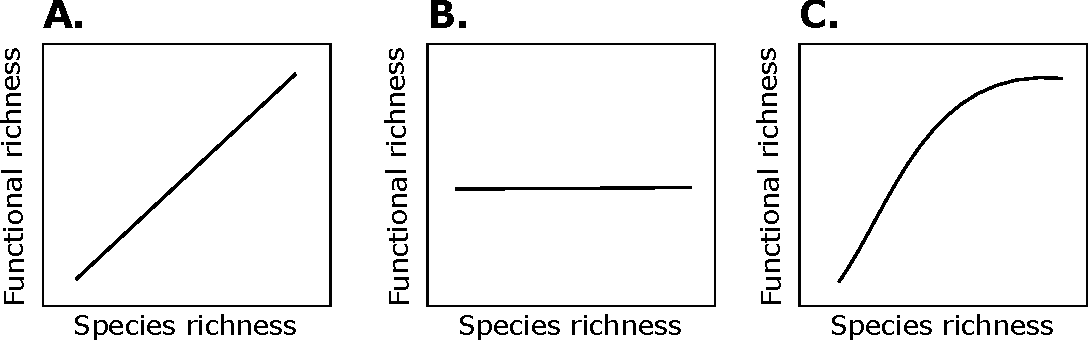
\includegraphics[scale=0.7]{figures/chapter1/Fredundancy.pdf}
\caption[The species richness -- functional richness relationship informs on functional redundancy.]{\textbf{The species richness -- functional richness relationship informs on functional redundancy.} \textbf{(A)} High positive correlation between species richness and functional richness: functional richness increases at a constant rate with species richness. The gain or loss of species can lead to marked variations in functional richness. The rate of increase is higher than in \textbf{(B)}, where functional richness remains constant despite variations in species richness. The functional redundancy of \textbf{(B)} is comparatively higher than that of \textbf{(A)}. \textbf{(C)} The rate at which functional richness increases with increases in species richness is not constant. The functional redundancy increases with higher species richness.} 
\label{fredundancy_ltr}
\end{figure}

The potential correlation of species richness with functional richness has two practical consequences. 

First, as underlined above, the shape of the relationship can inform on the functional redundancy of a given community (\cite{Cadotte2011}, and Figure \ref{fredundancy_ltr}). Thus, changes in the relationship between functional richness and species richness across a land-use gradient can provide insights into how land-use change impacts the functional redundancy of ecological communities. In assemblages with functionally redundant species, random species loss or addition are unlikely to lead to marked variation in functional richness.

Second, when species richness strongly correlates with functional richness (Figure \ref{fredundancy_ltr} A), decreases in functional richness along a land-use gradient may be due to decreases in species richness alone. In other words, an observed change in functional richness may be driven by changes in species richness alone rather than by environmental filtering. As such, it becomes necessary to disentangle the effects of species richness from the effects of the environmental variable of interest. To that end, a common approach consists in generating the null expectation of functional richness given a species richness. Then, empirical values can be compared against null expectations. This can be achieved through simulations where the community composition is randomised, given a species richness, so as to generate a null distribution of functional richness \citep{Wong2018, Flynn2009}.

\subparagraph{Functional dispersion.}
When a community is subject to environmental filtering, functional clustering is expected to be observed in the emergent community \citep{Wong2018, Cadotte2017}. Functional clustering -- also referred to as functional under-dispersion -- qualifies communities where species are more similar, in term of their traits, than expected by chance. Diverse indices have been developed to quantify the functional dispersion of ecological communities (for instance, Rao's quadratic entropy, or functional dispersion FDis, developed by \citet{Laliberte2010}). Rao's quadratic entropy and FDis aim at assessing the degree to which species resemble each other in terms of their traits. Chapter 3 provides more details on their definition and calculation (see Figure \ref{chartFDis}). 

Rao's quadratic entropy and functional dispersion are highly correlated. Both can be used to assess whether species in a given community are functionally clustered, as a consequence of environmental filtering. For instance, the observed dispersion in trait values can be compared to the null expectation of functional dispersion, obtained from a null model. As these indices are, by construction, independent from species richness, the effects of environmental filtering on functional dispersion can also be deduced directly from shifts in the values of the indices along an environmental gradient. 

As anthropogenic land-uses globally negatively impact local species richness \citep{Newbold2015}, decreases in functional richness of local ecological communities are likely to take place, particularly in communities with low functional redundancy. Moreover, land-use change could also alter the functional richness of communities without altering local species richness. For instance, \citet{Flynn2009} showed that the functional richness (DFR) of avian, mammalian and plant communities located in the Western hemisphere decreased under agricultural intensification. \citet{Chapman2018} showed that the functional richness (DFR) of tropical bird communities declined along a land-use gradient of increasing human disturbance. Other studies have reported shifts in the distribution of trait values along land-use gradients \citep{LaSorte2018, Rapacciuolo2017}. Overall, all these studies show that land-use change alters the functional richness of local vertebrate assemblages. Nevertheless, most studies were conducted at local or regional scales.

Some studies have been conducted at global scales to understand patterns in the functional dispersion of avian assemblages \citep{Cooke2019}, or in the functional richness (DFR) of mammalian communities \citep{Safi2011}. Nevertheless such studies did not focus on land-use change or other anthropogenic pressures, but on latitudinal gradients of species diversity. As such, to my knowledge, no study has yet investigated how land-use change impacts the functional diversity of local vertebrate communities at global scales. 

Studies looking at the effects of climate change on the functional diversity of terrestrial vertebrates are also rare. \citet{BarbetMassin2015} investigated how future climate change was projected to impact the functional diversity of global avian assemblages through range shifts. \citet{Thuiller2014} investigated how both projected land-use and climate change affected the functional diversity of European avian assemblages. Both studies highlighted that future range shifts due to climate change leaded to uneven effects on functional diversity across space, with some areas projected to experience substantial loss of functional diversity. To my knowledge, no work has investigated how future climate change is likely to impact the functional diversity of other vertebrate taxa (herptiles or mammals) at global scales. 

To summarise, past empirical evidence has shown that (1) species sensitivity to LUCC depends on their traits; (2) LUCC  is reshaping the functional composition of ecological assemblages, potentially disrupting important functions. Nevertheless, most studies have been conducted at local or regional scales, so that it is still unknown how global changes affect the functional diversity of local terrestrial vertebrate communities. Tackling this question, with land-use change at the disturbance of interest, is the aim of Chapter 3. 

The recent development of many functional diversity indices, synthesising the diversity of functions in a community, reflects the importance of understanding how anthropogenic pressures are likely to modify ecosystem processes. In the field of biodiversity-ecosystem functioning relationships, it is now well established that higher species diversity is associated with higher ecosystem productivity and stability, better use of limiting resource, as well as better resistance to biological invasions \citep{Tilman2014}. I now explore the links between functional diversity indices and ecosystem functioning in more details.

\paragraph{Functional diversity and ecosystem functioning}

Early experiments investigating the relationships between functional composition and ecosystem functioning classified species in broad functional groups. Species belonging to similar groups were assumed to have similar effects on ecosystem processes \citep{Legras2018}. Ecosystem functioning was measured in various ways, depending on the studied system. For instance, plant biomass was used to measure primary productivity in \citet{Weisser2017}. The field, overall, was dominated by experiments conducted on plant communities \citep{Tilman2014}, which are easier to manipulate and replicate than animal communities. A higher number of functional groups was correlated to better ecosystem functioning and resilience \citep{Tilman1994, Hector1999}. Consequently, the consensus that emerged was that higher levels of diversity meant higher ecosystem stability and performance; this idea is now widely accepted \citep{Hooper2005, Hooper2012, Oliver2015}. 

Conceptually, functional effect traits are the mechanistic links between biodiversity and ecosystem functioning \citep{Lavorel2002,Violle2007}. A higher diversity of effect traits induces increases in ecosystem performance, through, for example, more interspecific complementarity in resource use, or greater use of limiting resources \citep{Tilman2014}. Empirically, functional diversity indices have been found to be better predictors of ecosystem functioning than species richness \citep{Cadotte2011, Flynn2011, Abonyi2018}. Most studies looking at patterns of functional diversity now invoke this argument to justify the use of functional diversity indices. Researchers often claim that decreases in functional diversity indices could reflect the imperilment of ecosystem processes. Although this holds true for plants, for which there is a wealth of empirical evidence, the picture is more complex for animal communities. 

In animal communities, the use of functional diversity as a proxy for ecosystem functioning must be carefully justified. Indeed, there is to date little empirical evidence that functional diversity indices correlate with ecosystem processes supported by animal communities \citep{Hatfield2018, Didham2016}. For instance, in a meta-analysis of 24 studies looking at the effects of landscape change on functional diversity metrics, \citet{Hatfield2018} found that only five studies assessed whether functional diversity related to measures of ecosystem functioning. Moreover, these five studies overall found weak and contradictory associations between the functional metrics and the measures of ecosystem functioning. \citet{Hatfield2018} argued that, without empirical evidence of a strong link between functional diversity metrics and ecosystem processes, there is little incentive to continue to quantify the functional diversity of communities, in particular of animal assemblages.  \citet{Cadotte2011} also emphasized the need to clearly justify the use of functional diversity indices by showing that there is a correlation between functional indices and ecosystem functioning. Indeed, they argued that functional indices are worth measuring only if they provide with novel insights, compared to species richness, and if they reflect ecosystem function. Here, I acknowledge the points \citet{Hatfield2018, Cadotte2011}. Nevertheless, as exposed in the previous section, I argue that functional indices are still useful to document how global changes are altering the composition of animal communities. However, understanding how functional diversity indices relate to ecosystem functioning in animal communities is vital, and remains to be largely explored.

In animal communities, the use of functional diversity indices as proxies for ecosystem functioning is complexified by several elements that are less problematic in plant communities. First, ecosystem processes supported by animals may involve more than one taxon: for instance, both birds and arthropods impact pest control through predatory activity. \citet{Ewers2015} showed that, despite decreases in abundance in several invertebrate taxa between two land-uses, rates of decomposition, predation and seed consumption did not vary; vertebrate species compensated the loss of invertebrates by assuming similar functions at higher rates in altered land-uses. Therefore, the functional diversity of invertebrate species in this study could have been observed to decrease between the two land-uses, whereas no effect was observed on ecosystem functioning. 

Second, a single ecosystem process could arise from a combination of different traits, some of which difficult to measure. Appropriate trait selection is vital to ensure that functional diversity indices reflect targeted ecosystem functions \citep{Luck2012}. As emphasised by \citet{Didham2016}, the choice of functional traits must be mechanistically justified. However, the availability of trait data may be problematic, or traits could be difficult to measure. It may also be unclear which traits are more important in defining a given process. As such, the lack of correlation between functional diversity indices and ecosystem processes may arise from the difficulty to select and obtain appropriate traits in vertebrate communities. 

Finally, experimental set-ups in controlled conditions are much more difficult to put into place for terrestrial communities. It is extremely difficult to manipulate the composition of vertebrate communities, as is done in plant communities. Data is therefore mostly obtained from field studies, which may have confounding factors, including diverse taxa whose functional roles are neglected (with possibly, compensatory effects as underlined above, shown in \citet{Ewers2015}).

Overall, it remains largely unclear how the diversity and variability of vertebrate functional traits relates to ecosystem processes, despite the ecological importance of terrestrial vertebrates. If carefully designed functional diversity indices consistently related to ecosystem functioning, they would be relevant measures for the conservation of ecosystem processes and species.  

\subsection{Vertebrate ecological roles}
Vertebrate species play significant roles in ecosystem functioning, as they support a wide range of processes \citep{Sekercioglu2006, Severtsov2013, Hocking2014}. Vertebrates are also very important for human societies, both culturally and as sources of proteins \citep{Albert2018, Hirons2016,Alves2018}. Here, I briefly review the main ecological roles terrestrial vertebrate species participate in (mainly pollination, seed dispersal, predation, grazing and nutrient cycling).

First, vertebrate species participate in shaping global plant communities. The reproductive success of many plant species depends on vertebrates. Indeed, vertebrate species are significant pollinators \citep{Ratto2018}. Moreover, vertebrates are essential actors of seed dispersal. About 56\% of angiosperm species rely on biotic seed dispersal, either obligatory (14\%) or in complement to abiotic dispersal (42\%), and 46\% of gymnosperm species strictly rely on biotic seed dispersal \citep{Tiffney2004}. Vertebrates disperse seeds most frequently through endozoochory (ingestion of the disseminule or of part of the disseminule), and less frequently through exozoochory (where the disseminule gets attached to the surface of the disperser). Thus, through pollination and frugivory, vertebrates are important in maintaining gene flows among plant communities and impact the genetic diversity of plant assemblages \citep{Calvino-Cancela2012}.

By exerting top-down control, vertebrate grazers and herbivores regulate plant populations and influence global plant diversity patterns. \citet{Lin2018} and \citet{Zhang2018} both found global evidence that top-down interactions between vertebrates and plants shaped global plant communities. Mammalian seed predation contributes to the structure of tree communities \citep{Paine2016}. As ecosystem engineers (for example, through burrowing behaviours), vertebrates impact soil properties and influence the structure and the composition of plant assemblages \citep{Sekercioglu2006, Severtsov2013}.

Second, vertebrate species contribute to regulate animal populations through predatory activity \citep{Barber2010,Letnic2012, Luck2012, Salo2010}. Through both predatory and herbivory, vertebrates have a significant influence on the structure of food webs. 

Finally, vertebrate species participate in energy transfers between the biota and the abiotic environment. For instance, they take part in nutrient cycling and matter decomposition through scavenging \citep{Cunningham2018, Inger2016,Wilson2011}. Vertebrate excrements can modify nutrient availability in the soil, with cascading effects on the structure of plant communities \citep{Severtsov2013}.
  
To conclude, the range of ecosystem processes that vertebrate sustain is defined by their contribution to matter and energy flows at the ecosystem scale. Food webs are key to understand the transfer of matter and energy within the biota (interactions within and among trophic levels), from which multiple ecosystem properties emerge. Vertebrate species also contribute to mineralise organic matter, and as such participate in energy transfers between the biota and the abiotic environment. 


\subsection{Linking drivers of change and ecosystem functioning with the response-effect framework}
Efforts to link drivers of change and ecosystem function responses have been disparate across taxonomic groups, with a major focus on plants and invertebrates in the past years. Indeed, \citet{Hevia2017} showed in a metanalysis that most studies investigating how species traits mediate the impacts of stressors on ecosystem processes focused on plants and invertebrates, such that there is an existing taxonomic bias in this area. Vegetation and invertebrates both represented an approximate 40\% of the sampled papers, whereas only 17\% were dedicated to vertebrates. Their metanalysis also shed light on other biases, such as the spatial scale of the papers, with most sampled studies being conducted at local or national scales. Therefore, although terrestrial vertebrates have a major cultural, economic and functional importance and are over-represented in the overall biodiversity literature compared to other taxa \citep{Titley2017}, how disturbances affect the services they provide has not been extensively explored compared to other taxa. To understand how anthropogenic pressures may impact ecosystem processes sustained by vertebrate communities  at global scales, there is a need to assess whether LUCC significantly affects the functional diversity of vertebrate communities, and, in particular, the effect trait composition; and to verify whether effect trait composition predicts ecosystem processes, as detailed in the previous section (or, alternatively, apply this idea the other way around). 

The end-goal of the response-effect framework \citep{Lavorel2002, Naeem2003,McGill2006}, initially developed for plants, is to understand how environmental changes alter ecosystem functioning using response and effect traits. Indeed, if effect traits inform on ecosystem processes, response traits mediate species responses to environmental change. As such, the link between environmental pressures and ecosystem functioning is conceptually realised with both response and effect traits, when they overlap. The response-effect framework relies on identified response and effect traits to provide a mechanistic understanding of how disturbances modify the trait composition of communities, and how these changes link to alterations in functioning, driven by changes in the effect trait composition. 

The application of the response-effect framework to animal communities has been hindered by several issues \citep{Luck2012, Bartomeus2018, Didham2016}. For instance, there is a lack of empirical support for response and effect traits in animal communities; results may be contingent to a given taxon, hindering our ability to generalise predictions. 

\citet{Luck2012} underlined the need to develop robust and broadly applicable methods for vertebrates. They readapted the response-effect framework, with the aim to make it applicable for vertebrate species and provide guidelines for its application. Currently, our knowledge of how anthropogenic changes will alter the global processes sustained by vertebrate species is extremely limited, due to the diverse reasons exposed previously. One of the end-goal of my PhD project is to tackle this question at global scales and investigate whether the loss of certain trait combinations in response to LUCC may lead to the disruption of important ecosystem functions. As such, adaptations of the response-effect framework may be particularly relevant to this work.

To conclude, examining how vertebrate species traits influence their responses to LUCC is the first step to (1) elucidate which traits are likely to put species at greater risk, and find out whether it is possible to generalise patterns across vertebrate species  (by working at global scales and comparatively across the four terrestrial vertebrate classes); (2) investigate whether future biodiversity declines triggered by these anthropogenic changes are likely to disrupt important ecosystem functions. 

The work I have achieved so far focuses on land-use change at global scales and aims at investigating the questions detailed in the next section.


\section{Questions and hypotheses investigated in the present report}
Here, I briefly introduce the questions I tackled in this report. They will be developed in more detail in each corresponding Chapter.

\subsection{Chapter 2: Collecting and imputing ecological traits across terrestrial vertebrates}

As underlined in the introduction, functional traits can provide a mechanistic understanding of how environmental stressors affect both ecological assemblages and ecosystem processes. As such, they convey information most relevant to conservation policies. According to \citet{Hekkala2018}, global assessments of how land-use change affects vertebrate functional diversity may have been limited so far by the amount of ecological information required to conduct such analyses, notably by the availability of species traits. There exist published databases of species traits, many of which quite recently published (see Table \ref{datasources} in Chapter 2), but despite these collation efforts, some taxa are likely to remain under-sampled. For this project, I collate information on vertebrate traits prior to conducting any analysis (Chapter 2). I assess the gaps in trait information across terrestrial vertebrates and investigate whether trait information present taxonomic, phylogenetic and spatial biases. Notably, I hypothesize that:
 \begin{itemize}
\item Mammals and birds are, overall, better sampled than herptiles;
\item Species with larger range sizes are more likely to have more complete trait information;
\item Trait data is phylogenetically biased: closely related species are more likely to have a similar amount of available trait information than less related species.
\end{itemize}

After assessing the gaps in the availability of trait information, I impute missing trait values using random forests algorithms. All traits are used as predictors in the process. Phylogenetic information is incorporated as an extra predictor in the form of phylogenetic eigenvectors. I then evaluate imputation performance and congruence. 

Next, the compiled trait dataset is used for further analyses (Chapter 3). In Chapter 3, I address the questions presented in the section below.

\subsection{Chapter 3: Land-use change promotes the functional homogenisation of local vertebrate communities}

The aim of this Chapter is to investigate how land-use change affects the functional diversity of vertebrate communities. Because obtaining longitudinal information on compositional changes can be difficult, the effects of land-use change throughout this project are studied using a `space-for-time' substitution, whereby a spatial gradient is used as a proxy for temporal dynamics \citep{depalma2018}. As such, the following analyses  build upon the PREDICTS database, a large collated dataset of species occurrence and abundance around the world across different land-uses \citep{Hudson2014, Hudson2017}. To date, this database constitutes the most comprehensive global collection of biodiversity samples across different land-uses. It comprises 666 studies, each of which recording the occurrence and/or abundance  of species at different sites (abundance in most cases). Each site is classified into a land-use category; land-use categories encompass primary vegetation, secondary vegetation, plantation forest, cropland, pasture and urban. Primary vegetation refers to native vegetation undisturbed since its development under current climatic conditions. Where primary vegetation was destroyed (either by human actions or natural causes), recovering vegetation forms are referred to as secondary vegetation. Secondary vegetation is further divided into three categories: mature, intermediate and young, depending on the stage of recovery of the vegetation.
Finally, plantation forest, cropland and pasture refer to agricultural areas (crop trees grown for human purposes, biofuels and herbaceous crops, and areas grazed by livestock).

Using this database, I aim to investigate how land-use change impacts the functional diversity of local vertebrate communities. I hypothesise that by reducing local habitat heterogeneity, human-dominated land-uses promote functional homogenisation and clustering, whereby the similarity in trait composition across assemblages increases through the loss of certain functions. This hypothesis relies on the idea that strong environmental filtering will disproportionately remove certain functional types. To test this hypothesis, I use various indices of functional diversity. Specifically, I calculate the two indices of functional richness presented earlier in this Chapter: volume-based functional richness FRic \citep{Villeger2008} and dendrogram-based functional richness DFR \citep{Petchey2002}. Below, I state the hypotheses for these indices.
\begin{itemize}
\item Where functional richness indices are not correlated with species richness, I expect functional richness to decrease in more human-dominated land-uses, with habitat filtering reducing the amount of utilised trait space. 
\item When species richness is correlated with functional richness, I expect the slope of the species richness--functional richness relationship to be smaller in more disturbed land-uses (this hypothesis links to the hypothesis on functional redundancy presented further down; Figure \ref{fredundancy_ltr}). 
\end{itemize}

I also calculate the functional dispersion \citep{Laliberte2010} of each local community. Finally, I use an index developed by \citet{Ricotta2016} to estimate functional redundancy. This index combines Rao's quadratic entropy and the Gini-Simpson diversity index. Specifically:
\begin{itemize}
\item I expect functional dispersion to decrease with increasing land-use disturbance, with species within human-dominated land-use communities presenting more similar trait values, due to functional clustering.
\item I expect more disturbed land-uses to have higher degrees of functional redundancy, as the similarity in functional composition increases across species.    
\end{itemize}

These constituted the hypotheses for the work presented hereafter. In Chapter 4, I detail some questions that I aim to investigate in the future years of my PhD. All analyses and data collation were conducted using R \citep{R_citation}.

\chapter{Collecting and imputing ecological trait data across terrestrial vertebrates}
\section{Introduction}

A growing body of research uses trait-based approaches to understand how biodiversity links to ecosystem functioning, and how environmental changes are likely to affect species non-randomly with respect to their traits (Hevia et al). Strictly, traits are defined as characteristics measurable the level of an individual, with an effect on organismal fitness or performance. They can be physiological (e.g., metabolic rates), morphological (e.g., body mass), behavioural (e.g., learning) or phenological (e.g., anthesis), or can relate to species life-history (e.g. longevity). This definition can be broadened to include characteristics measurable at the species level, such as the number of habitats known to be used by a species (habitat breadth). Here, I use this broader definition of traits and refer to these as ecological traits.

Many studies have shown that traits influence species responses to environmental pressures (). Moreover, it is now accepted that ecosystem functioning is positively correlated with species functional diversity (Tilman). Species traits can provide a mechanistic understanding of both species roles in ecosystem functioning and of species responses to changes. Traits shape species fundamental and realised niches; for instance, physiological traits influence species thermal tolerances, participating in defining their geographical distributions. Traits such as trophic level or body mass structure food webs and affect inter- and intra-specific competition. As such, traits determine and reflect species use of their environment. Specifically, effect traits define organismal contributions to ecosystem functions. Effect traits are underpinned by species resource use, and this applies at diverse scales, from single-celled nutrient cycling bacteria to large mammals. Response traits are those involved in determining species responses to environmental changes and can overlap with effect traits. 

Although terrestrial vertebrates have been extensively studied in the past (Titley et al), the vast majority of research investigating the impact of environmental changes on ecosystem functions has focused on plants and invertebrates (Hevia et al). Vertebrates nevertheless play diverse ecosystem roles, and some are important keystone species.  Vertebrate species particularly contribute in food web structures and population dynamics through predatory and herbivory activity. They are pollinators and seed dispersers, and overall participate in nutrient cycling at higher levels. Understanding how environmental changes may affect their ecological roles is important to predict future ecosystem functioning, and to put into place appropriate mitigation measures. The end-goals of my PhD thesis are to elucidate how species traits influence their responses to land-use and climate change, and how this links to changes in ecosystem functioning. Addressing these questions requires to use extensive trait data. Despite vertebrates having been the focus of much research, and despite the growing interest for trait-based approaches, there exist no comprehensive database of vertebrate ecological traits encompassing all classes. Consequently, collating trait data was a prerequisite for any further work, and this operation was constrained by the amount of information available in the literature. The present chapter focuses on data collection methods and missing trait values imputations. Thanks to past and recent efforts to release data in the public domain, at least four comprehensive ecological trait databases are now freely accessible (mammals: Pantheria, amphibians: Amphibio, amniotes: Myhrvold, mammals and birds: Cooke et al). Other trait datasets have been released on online platforms alongside published articles (e.g. Global Assessment of Reptile Distribution initiative, \url{http://www.gardinitiative.org/}), or can be downloaded from online databases (IUCN Red List (\url{https://www.iucnredlist.org/}), BirdLife data zone (\url(http://datazone.birdlife.org/home)). Trait data available from primary sources for mammals and birds is likely to be more abundant and more resolved than for reptiles and amphibians, due to systematic biases in sampling with regards to taxonomic groups (Newbold, \textit{manuscript}).

The present chapter details the methodology I employed to collate trait information across terrestrial vertebrates. Primary sources offered a variety of traits, of which only a few were selected. Trait selection was motivated by two main reasons: (1) traits should be of ecological interest and be related to response or effect processes; (2) trait values should be available for many species, across the four terrestrial vertebrate classes, allowing for cross-classes comparative analyses. The selected target traits related to species life-history and morphology (body mass; longevity; litter/clutch size; diel activity; trophic level; diet) and to their habitat preferences (habitat breadth and specialisation). Reptilian diet was not readily available in primary data sources, and one exception was made as I extracted diet data for the other classes. Species mobility was hardly available across sources, and no similar variable could describe species mobility across classes; although species' abilities to move in their environment is likely to strongly impact their responses to threats, this trait was not considered for the above reasons. 

The present chapter details the methodology I employed to collate selected traits. I elaborate on some of the challenges met when compiling data across many species, such as inconsistency of taxonomy across sources. Not unexpectedly, the amount of missing values was highly variable across classes and traits. To achieve full trait coverage across species, I imputed missing trait values using random-forest algorithms.
In this chapter, I briefly examine imputation performance, notably by assessing whether increasing species representation in phylogenetic trees affects imputation error. 

In October 2018, Cooke et al released a comprehensive database of six mammalian and avian traits. They collated and imputed missing trait values for body mass, litter/clutch size, volancy, diel activity, primary diet and habitat breadth. As similar primary sources were used in both our data collection, I did not use their database to complement my sources. Moreover, the imputation methods they used to fill gaps in trait coverage differed from mine. I used this freely accessible compiled data as an opportunity to compare the results of both our data collection and imputation processes. This chapter also presents results from this comparison (more extensively so in the SI).

Finally, the trait data collected and imputed in this chapter can be subject to future changes, and may not final at this stage.

%Finally, I briefly examine patterns in missing values with regards to species phylogenetic position.




\pagebreak
\section{Methods}

\subsection{Ecological trait data collection}

\subsubsection{Primary data sources.}
I collated ecological trait data for terrestrial vertebrates from the sources figuring in Table \ref{datasources}. Information was compiled for the following target traits: body mass, longevity, litter or clutch size, trophic level, diel activity, diet, and habitat preferences. I also compiled traits that were potentially correlated to either body mass or longevity, to be used as potential predictors in imputations of missing values. As such, body length information was compiled when available, as well as generation length or age at sexual maturity. Most notably, longevity was chosen over generation length or age at sexual maturity as it was the only common currency across classes reflecting generation turnover. In addition, species geographical range sizes were estimated from distribution data, extracted from the IUCN Red List.

% Table of sources.
\begin{table}[h!]
\renewcommand{\baselinestretch}{1}
\renewcommand{\arraystretch}{1.5}
\begin{center}\fontsize{9}{11}\selectfont
\caption[Primary sources used for each compiled trait.]{\textbf{Primary sources used for each compiled trait.} Primary sources may contain more traits than shown here. \textbf{BM}: body mass; \textbf{BL}: body length; \textbf{L}: longevity or maximum longevity; \textbf{GL}: generation length; \textbf{LCS}: litter or clutch size; \textbf{TL}: trophic level; \textbf{Di}: diet; \textbf{DA}: diel activity; \textbf{RS}: range size; \textbf{H}: habitat data. Bolded abbreviations highlight target traits; other traits were added for potential correlations in further imputations.} 
\label{datasources}
\begin{tabular}{|l|c|c|c|c|c|c|c|c|c|c|c|c|}
\hline
\multicolumn{1}{|c|}{\multirow{2}{*}{\textbf{Sources}}} & \multirow{2}{*}{\textbf{Taxa}} & \multicolumn{9}{c|}{\textbf{Traits}} & \multirow{2}{*}{\textbf{RS}} & \multirow{2}{*}{\textbf{H}} \\ \cline{3-11}
\multicolumn{1}{|c|}{} &  & \textbf{BM} & BL & \textbf{L} & MA & GL & \textbf{LCS} & \textbf{TL} & \textbf{Di} & \textbf{DA} &  &  \\ \hline
Amphibio & \multirow{4}{*}{Amphibians} & \checkmark & \checkmark & \checkmark & \checkmark &  & \checkmark & \checkmark & \checkmark & \checkmark &  &  \\ \cline{1-1} \cline{3-13} 
Cooper &  &  & \checkmark &  &  &  & \checkmark &  &  &  & \checkmark &  \\ \cline{1-1} \cline{3-13} 
Senior &  &  & \checkmark &  &  &  &  &  &  &  &  &  \\ \cline{1-1} \cline{3-13} 
Bickford &  &  & \checkmark &  &  &  &  &  &  &  & \checkmark &  \\ \hline
Elton & \multirow{2}{*}{Birds} & \checkmark &  &  &  &  &  &  & \checkmark & \checkmark &  &  \\ \cline{1-1} \cline{3-13} 
Butchart &  & \checkmark &  &  &  & \checkmark &  &  &  &  &  &  \\ \hline
Pantheria & \multirow{5}{*}{Mammals} & \checkmark & \checkmark & \checkmark & \checkmark &  & \checkmark &  &  & \checkmark &  &  \\ \cline{1-1} \cline{3-13} 
Kissling1 &  &  &  &  &  &  &  & \checkmark &  &  &  &  \\ \cline{1-1} \cline{3-13} 
Kissling2 &  &  &  &  &  &  &  & \checkmark &  &  &  &  \\ \cline{1-1} \cline{3-13} 
Elton &  & \checkmark &  &  &  &  &  &  & \checkmark & \checkmark &  &  \\ \cline{1-1} \cline{3-13} 
Pacifici &  & \checkmark &  & \checkmark & \checkmark & \checkmark &  &  &  &  &  &  \\ \hline
Scharf & \multirow{8}{*}{Reptiles} & \checkmark &  & \checkmark & \checkmark &  & \checkmark & \checkmark &  & \checkmark &  &  \\ \cline{1-1} \cline{3-13} 
%Meiri &  &  &  &  &  &  &  & \checkmark &  & \checkmark &  &  \\ \cline{1-1} \cline{3-13} 
Vidan &  &  &  &  &  &  &  &  &  & \checkmark &  &  \\ \cline{1-1} \cline{3-13} 
Stark &  & \checkmark &  & \checkmark &  &  & \checkmark &  &  & \checkmark &  &  \\ \cline{1-1} \cline{3-13} 
Schwarz &  &  &  &  &  &  & \checkmark &  &  &  &  &  \\ \cline{1-1} \cline{3-13} 
Novosolov1 &  & \checkmark &  &  &  &  &  & \checkmark &  &  & \checkmark &  \\ \cline{1-1} \cline{3-13} 
Novosolov2 &  &  &  &  &  &  & \checkmark &  &  &  &  &  \\ \cline{1-1} \cline{3-13} 
Slavenko &  & \checkmark &  &  &  &  &  &  &  &  &  &  \\ \hline
Myhrvold & Amniotes & \checkmark & \checkmark & \checkmark & \checkmark &  & \checkmark &  &  &  &  &  \\ \hline
IUCN & Vertebrates &  &  &  &  &  &  &  &  &  & \checkmark & \checkmark \\ \hline
\end{tabular}
\end{center}
\end{table}

\subsubsection{Compilation methods.}

\paragraph{Continuous traits.}
All continuous traits were averaged within species when different sources provided estimates. Longevity and maximum longevity were assumed to provide the same information and were averaged within species. No measure of intra-specific variability was compiled and estimates were provided as a single measure for each species.

\paragraph{Categorical traits.}
\subparagraph{Activity time.}
Species were described as being either nocturnal or non-nocturnal. Despite a higher resolution of activity time information in some of the primary sources (e.g. species being described as cathemereal, crepuscular or strictly diurnal), I adopted the classification of the primary source with the lowest resolution, in order to have consistent information across classes.
\subparagraph{Diet and diet breadth.}
For mammals and birds, diet was compiled from the Elton Traits database (ref). Primary diet was available in the avian dataset and declined into five categories: (1) plant or seed consumers; (2) fruit or nectar consumers; (3) vertebrate consumers, including fish and carrion; (4) invertebrate consumers; and (5) omnivores. Primary diet was not available for mammals. Instead, mammal diet was only described as the percent use of different food items. I pooled these items together into the same five primary diet categories as for the avian dataset. Any food items for which percent use was equal to or above 50\% were considered to be primary food items. Species for which no food item had percent use above 50\% were considered to be omnivores.\\ 
For amphibians, diet information was extracted from AmphiBIO. Diet information was available as binary variables for diverse food items. Percent use were not recorded, so these items were considered to form species primary diet. I pooled amphibian species into the five diet categories described above.
\subparagraph{Trophic level.} For amphibians and birds, trophic levels were partly inferred from the primary diet. 
\subparagraph{Habitat preferences.}
Species habitat preferences were compiled from IUCN habitat data files and were described as a binary variable recording whether a species was known to occur in a particular habitat. I calculated habitat breadth as the number of habitats a species was known to use. Weights were assigned to each habitat in this calculation depending on the recorded habitat suitability and importance; outcomes were not very sensitive to the presence of weights (compared to a non-weighted sum, see SI). Finally, a broad degree of habitat specialisation was produced. If any artificial habitat was recorded to be suitable, species were reported to be generalists; else, they were natural habitat specialists. More details on habitat preferences compilation are provided in the SI. 

\subsection{Phylogenetic information}
I obtained phylogenetic trees for birds, amphibians, mammals and squamates from Hedges et al (2015) (available at \url{http://www.biodiversitycenter.org/ttol}, downloaded 06/07/2018). All trees were ultrametric and fully resolved, except for the amphibian tree which presented polytomies. All trees contained a few branches of length 0 (193 branches for mammals, 136 for amphibians, 189 for birds and 284 for reptiles).

\subsection{Tackling taxonomic synonymy}
Across the different primary sources, similar species could appear under different binomial names. This was a problem when matching datasets by species. It was also problem when matching species to the PREDICTS database. Moreover, it is possible than within a primary source, a given species was appearing under two or more different names. As such, taxonomic synonymy created `pseudoreplicates' of the same species, overall falsely increasing the total number of species and artificially inflating the amount of missing trait values. Taxonomic synonymy was hence a major issue; due to the large number of species across datasets, extensive manual checks could not be applied. The presence of typos in species names had the same effect as synonymy, erroneously duplicating species. I attempted to correct for taxonomy first by correcting for typos, and second by identifying species which were entered under a synonymic name and replacing these with the accepted name. To this end, I developed an automated procedure, complemented with a few manual entries. Obvious cases where vernacular names had been entered in the place of binomial names were also treated manually; that was the case for 44 PREDICTS species (when possible, I best assigned binomial names to species common names; unidentifiable species were left empty and assigned to a genus (5 species)).

\subsubsection{Automated procedure and outputs.}
\paragraph{Extracting names from the IUCN Red List and the Integrated Taxonomic Information System (ITIS).}
The automated procedure consisted in extracting species accepted and synonymic binomial names from the IUCN Red List or from the ITIS, using the rredlist and taxize R packages. I started by generating a list of all names figuring across datasets (primary sources, phylogenies and PREDICTS). These `original' names were corrected for typos; then, the IUCN Red List was queried and synonyms and accepted names were stored when possible. When species were not found in the IUCN Red List, information was extracted from ITIS. When species were not found in ITIS either, corrected names were assumed to be accepted. Family and order information was extracted using the same procedure and some entries were completed using the Global Biodiversity Information Facility taxonomic backbone (\url{https://www.gbif.org/tools/species-lookup}).\\
\textbf{NB:} for species entered with the forms \textit{Genus cf.}, \textit{Genus aff.} or \textit{Genus spp.}, the accepted name was left empty.

\paragraph{Outputs.} I generated a list of vertebrate species, recording whether species names were accepted or synonymic (for 14124, 8743, 6090, and 11183 names or identifiers found across datasets for birds, amphibians, mammals and reptiles respectively, including species names as they appeared in phylogenetic trees). For each name, the identified accepted name and the synonyms were stored when possible, as well as additional taxonomic information (order, family, genus). When queries did not succeed, species accepted names were assumed to be the original names found in the datasets.

\paragraph{Harmonising taxonomy in trait datasets.}
Taxonomy across datasets was finally homogenised by replacing recorded synonyms with their accepted scientific names. Overall, this procedure  reduced the total number of species figuring in trait datasets (Figure \ref{taxcor}). The species presenting the highest degree of pseudoreplication was the East African mole rat (\textit{Tachyoryctes splendens}), which was figuring under 12 names identified as being synonymic across primary sources (Figure \ref{taxcor}B), highlighting the need for normalising taxonomy across sources.

% figure: distribution of names and differences in species number
\vspace{0.5cm}
\begin{figure}[h!]
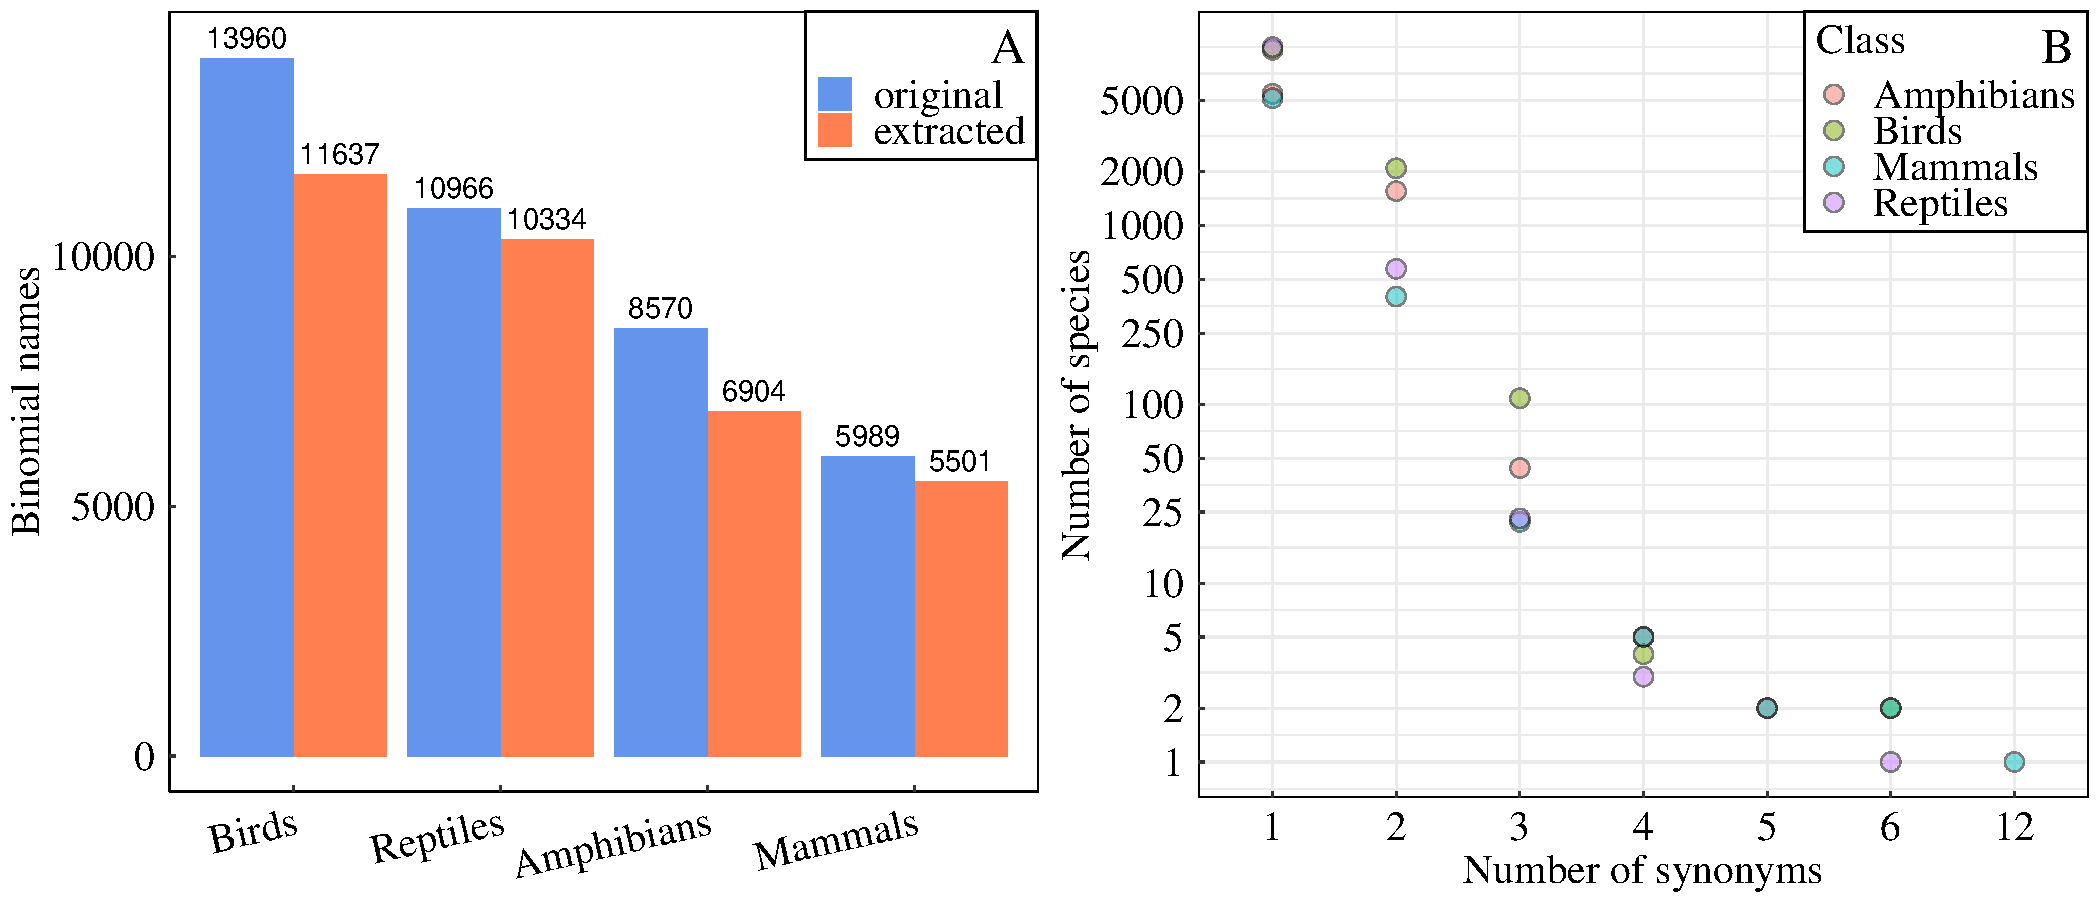
\includegraphics[scale=0.45]{figures/chapter2/Taxonomic_corrections/tax_corrections}
\caption[Difference in species number due to taxonomic correction (A) and distribution of number of synonyms across datasets (B)]{\textbf{Difference in species number due to taxonomic correction (A) and distribution of number of synonyms across datasets (B).} \textbf{(A)} shows the number of species across all primary sources (trait datasets and PREDICTS, excluding phylogenies), before and after correcting for taxonomy. Replacing identified synonyms by the extracted accepted name reduced the number of species in all classes, with the most drastic reduction for birds (decrease by 2,323 unique binomial names). The diminution was of 632 unique identified species for reptiles, of 1,666 for amphibians and of 488 for mammals. \textbf{(B)} shows the distribution of the number of synonymic names. In all four classes, more than 5,000 species (or binomial names) had no identified synonyms. Nevertheless, a large amount of species had two identified synonyms (range: 400 species for mammals - 2086 for birds). The most replicated species was the East African mole rat \textit{Tachyoryctes splendens}, for which 11 synonyms were identified.}
\label{taxcor}
\end{figure}

Despite the automation efforts, taxonomic redundancy persisted to a degree in the trait datasets. Indeed, at this stage, not all species in PREDICTS matched a species in the trait datasets. Additional manual inputs were required to resolve taxonomic synonymy for these species. Verifying the presence of PREDICTS species in trait datasets was important for further analyses. Taxonomic synonymy was resolved manually for 91 PREDICTS species that did not match any species in the trait datasets; in that case, information was extracted from other diverse sources (such as the Reptile Database (\url{http://www.reptile-database.org/}); Avibase (\url{https://avibase.bsc-eoc.org/avibase.jsp?lang=EN&pg=home}); AmphibiaWeb (\url{https://amphibiaweb.org/})). After adding manual inputs to the synonym datasets, all PREDICTS species were represented in trait datasets. 

The need to apply additional manual inputs underlines the fact that the automated procedure was not optimal. The Red List and the ITIS were not comprehensive taxonomic sources, and for clades with high degrees of pseudoreplication in names, such as reptiles or amphibians, neither the Red List or the ITIS were fully resolved. As I only applied manual checks for PREDICTS relevant species, `pseudoreplication' and taxonomic errors are likely to have persisted to a degree. Moreover, certain species were entered using the format \textit{Genus subspecies} rather than \textit{Genus species}; for these, automated queries may have failed to identify the species.

% Extract of synonym dataset? in the SI


\subsubsection{Harmonising taxonomy in phylogenetic trees and increasing species phylogenetic representation.}

\paragraph{Taxonomic correction across tip labels.} 
Efforts to correct datasets for taxonomy created problems for a marginal proportion of species when dealing with phylogenies. The idea of the procedure described above was to replace two or more identified synonyms by a single accepted name, and then collapsing dataset rows together by names. I applied the same method on phylogenies, replacing synonyms by their identified accepted names in trees' tip labels. Not unexpectedly, in some cases, the procedure ended up assigning the same accepted name to different phylogenetic tips. This was the case for 2.8\% of mammalian, 1.7\% of avian, 1.6\% of amphibian and  1.7\% of reptilian species, which then had multiple phylogenetic positions (most having two different positions, see SI). Because keeping several putative phylogenetic positions for a species was problematic in further analyses, I selected one tip to conserve and dropped other tips from the phylogenies (Figure \ref{chart_phylorep}). To briefly describe the procedure, if replicated tips were sister clades, the tip to conserve was chosen randomly among the replicates. Else, I chose to conserve the tree tip whose position was closest to the position of the same tip in the uncorrected tree, when present. In all other few cases, tips to drop were chosen randomly. Further details on how replicated tips were dropped are available in the SI (with 3 examples for each case of Figure \ref{chart_phylorep}).

\begin{figure}[h!]
\centering
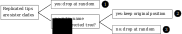
\includegraphics[scale=0.7]{figures/chapter2/chart_phylorep}
\caption[Procedure followed to drop replicated tips from phylogenies]{\textbf{Procedure followed to drop replicated tips from phylogenies.} Most of these were replicated twice. When replicated tips were sister clades, the tips to drop were chosen randomly, as it did not affect the `true' phylogenetic position of the species (1). When replicated were not sister clades, I kept the tip whose position was closest to the position of the same tip in the uncorrected tree (2). In a few cases, the corrected name did not appear in the original tree. Those were problematic cases, and the tips to drop were chosen randomly (3). Nevertheless, occurences of that third case were rare (see SI).}
\label{chart_phylorep}
\end{figure}

% Table with number of replicates, number of which were sister clades:
% Number of repliated tips, number that are sister clades, number that are truly pbmatic
% occurences of number of replicates.
\begin{figure}[h!]
\centering
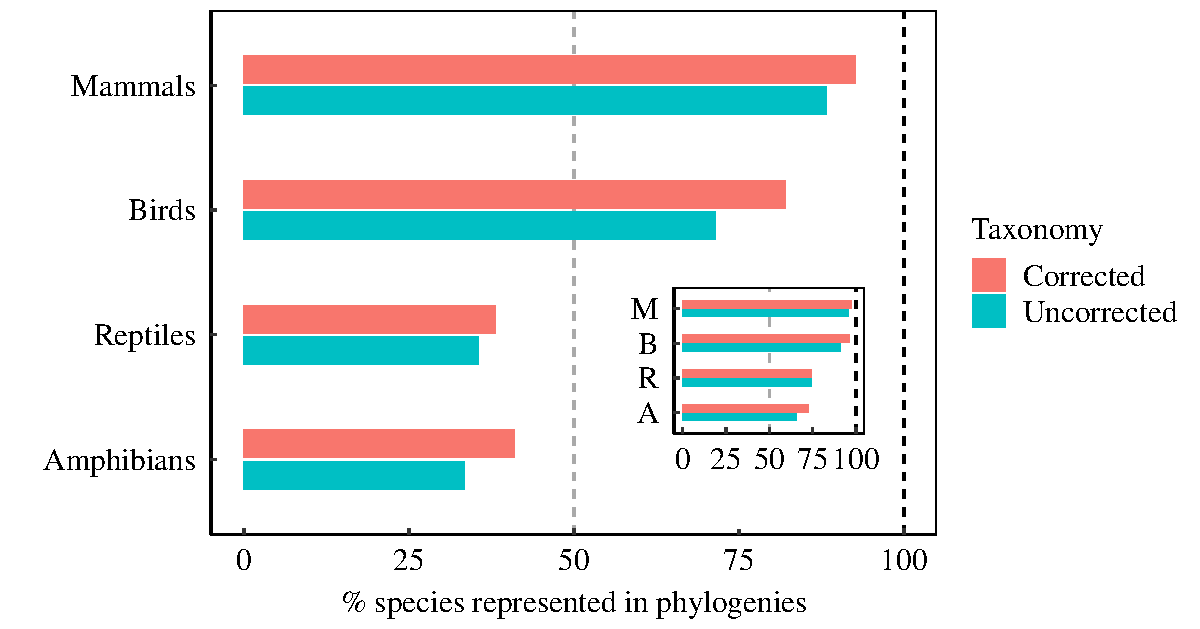
\includegraphics[scale=0.7]{figures/chapter2/Species_representation_phylo}
\caption[Percentage of species represented in the phylogenies for both corrected and uncorrected trait datasets]{\textbf{Percentage of species represented in the phylogenies for both corrected and uncorrected trait datasets.} Overall, taxonomic correction increased species representation in phylogenetic trees. Representation for mammals and birds was high (after taxonomic correction: 82\% of avian and 93\% of mammalian species had a phylogenetic position). On the other hand, reptiles and amphibians were poorly represented (after taxonomic correction: only 38\% of reptilian and 41\% of amphibian species were placed in phylogenetic trees). The inset barplot shows representation for species figuring in PREDICTS. For these, species presence in phylogenetic trees after correction was high across all classes, with a minimum representation of 76\% for amphibians.}
\label{species_rep_phylo}
\end{figure}

\paragraph{Correcting for taxonomy in the phylogenies: conclusions.}
Overall, correcting for taxonomy in phylogenies improved species representation in the trees (Figure \ref{species_rep_phylo}. For amphibian and reptilian species figuring in PREDICTS only, phylogenetic representation disproportionally increased (with a minimum representation of 76\% for PREDICTS amphibians after correcting the trees for taxonomy, inset plot in Figure \ref{species_rep_phylo}). Nevertheless, correcting phylogenetic tip labels generated replicates for a marginal number of tips, which then had to be dropped. 


\paragraph{Species attachments to phylogenetic trees.} Some species in the trait datasets were not represented in the phylogenies. Maximising the number of species represented in the phylogenies was important for further trait imputations. Indeed, if traits were evolutionary conserved, species phylogenetic position could be an important predictor of trait values. To maximise species representation, I added some species to the root of their genus, when possible (phytools package). Attaching species at the root of their genus created polytomies, which were resolved randomly (using multi2di, ape package). Resulting trees contained branches of length zero. To facilitate further analyses, a small number ($10^{-10}$) was added to these branch lengths; consequently, the trees were not ultrametric.  were Such a process could have altered the significance and the strength of trait phylogenetic signal. I further verify whether these alterations of the trees had impacted phylogenetic signal, by qualitatively comparing the strength and the significance of phylogenetic signal for each trait estimated using both original trees and augmented trees (see `Assessing phylogenetic signal in traits').

A large number of species were attached to their genera in the trees (Table \ref{random_attachments_phy}); for instance, only 38\% of the species figuring in the reptilian trait dataset were initially found in the squamate phylogeny. After attaching non-represented species, 91\% of the species were placed in the squamate phylogeny. 

\begin{table}[h!]
\renewcommand{\baselinestretch}{1}
\renewcommand{\arraystretch}{1.5}
\begin{center}\fontsize{9}{11}\selectfont
\caption[Species representation in phylogenetic trees (corrected taxonomy)]{\textbf{Species representation in phylogenetic trees (corrected for taxonomy).} The number of species attached to the root of their genus ranged from 175 (mammals) to 5438 (reptiles). Finally, most species were represented in the phylogenies, whereas more than half reptilian and amphibian species initially had no known phylogenetic position.} 
\label{random_attachments_phy}
\begin{tabular}{|l|l|l|c|l}
\cline{1-4}
\multicolumn{1}{|c|}{\textbf{Class}} & \multicolumn{1}{c|}{\textbf{Initially not in tree}} & \multicolumn{1}{c|}{\textbf{Of which randomly attached}} & \textbf{No final representation in tree} &  \\ \cline{1-4}
Amphibians                  & 59\% (4040 of 6904)                           & 96\% (3883 of 4040)                     & \textbf{2.3\%}             &  \\ \cline{1-4}
Birds                       & 18\% (2085 of 11637)                          & 75\% (1574 of 2085)                    & \textbf{4.4\%}             &  \\ \cline{1-4}
Mammals                     & 7.4\% (407 of 5502)                           & 43\% (175 of 407)                       & \textbf{4.2\%}            &  \\ \cline{1-4}
Reptiles                    & 62\% (6391 of 10334)                          & 85\% (5438 of 6391)                    & \textbf{9.2\%}             &  \\ \cline{1-4}
\end{tabular}
\end{center}
\end{table}


\subsection{Exploring biases in the coverage and completeness of trait information across classes}
Having normalised taxonomy and compiled trait data, I assessed trait coverage, defined as the percentage of species for which trait information was available for a given trait. To estimate the amount of trait information available for a species, I calculated trait completeness. For a species, trait completeness was defined as the proportion of traits for which information was available (number of non-missing trait values divided by total number of traits). In corrected datasets, species with 0\% completeness in predictor traits were filtered out.

Further, I examined whether patterns in the distribution of missing values emerged within classes, as particular clades or parts of the phylogenies could be under-sampled compared to other clades.
Whether values are missing at random is likely to impact imputation errors, notably if some taxa are under-sampled compared to others. To assess whether missing values presented patterns, I plotted within-family median completeness and coverage values in each branches of phylogenetic trees built at the family level. Tree branches were colour-coded to reflect the median value in each family. Specifically, within family trait completeness was calculated by aggregating species into their families and calculating the median trait completeness within each group. 
Patterns of missing values in trait coverage were explored for each trait separately. Trait coverage was assessed within families as the number of species for which values were missing over total number of species in each family. As families represented by very few species might present higher percentages of missing values, reflecting family size rather than randomness in sampling, I contrasted trait coverage plots against a plot showing how much each family contributed to the total number of species (number of species in each family over total number of species in the tree).


\subsection{Imputing missing trait values}
In order to achieve full trait coverage across classes, I imputed missing trait values. Diverse imputation methods have been developed and used in published articles. Penone et al (2014) assessed the performance of four different imputation approaches (K-nearest neighbour (kNN, Troyanskaya 2001), multivariate imputation by chained equations (mice, van Buuren 2009, 2011), random forest algorithms implemented with missForest (Stekhoven, 2011) and phylogenetic imputations implemented with phylopars (Goolsby, 2016)). Their study showed that the kNN approach resulted in significantly higher imputation errors than the three other approaches. Both missForest and phylopars were the best methods when phylogenetic information was included. Nevertheless, phylopars was much slower than missForest, and could only handle continuous traits. missForest was faster and could deal with mixed type data. Without phylogenetic information, mice was found to be the best method, with fast imputations of mixed-type data. Of all these methods, missForest was the only one that did not make assumptions about data distribution (being a non-parametric approach), or that did not require a prior knowledge of some tuning parameters. As such, missForest appeared to be an interesting option for missing data imputation. To further assess whether to use random forests rather than multivariate chained equations, I estimated the phylogenetic signal in traits. Strong phylogenetic signal in traits would indicate than missForest could perform better than mice.

\subsubsection{Assessing phylogenetic signal in traits}

\paragraph{Measuring phylogenetic signal in continuous traits with Pagel's $\lambda$.}
Phylogenetic signal is a measure of the tendency of closely related species to resemble each other more than less related species. Diverse statistics have been developed to estimate phylogenetic signal, most of them applying to continuous traits (Munkemuller 2012). I used Pagel's $\lambda$ (function phylosig, phytools package). Pagel's $\lambda$ is a scaling component that measures the coefficient by which the trait covariance matrix should be weighted to fit a Brownian motion model of evolution. Indeed, under a Brownian motion model of evolution, the trait covariance matrix is expected to be influenced only by the phylogenetic history: changes in trait values happen at random and trait variance is proportional to evolutionary time. When other factors are at play, the observed covariance matrix is the expected covariance matrix transformed with the estimated $\lambda$. A value close to 0 indicates that the covariance matrix need not be transformed by much to fit a Brownian motion. On the other hand, a value close to 1 indicates that trait values are more similar in closely related species than expected under a Brownian motion model of evolution. Using Pagel's $\lambda$, I assessed the strength of the phylogenetic signal. The phylosig function (phytools) also allows to test for signal significance (comparing the estimated $\lambda$ to the null expectation of $\lambda$ with a log-likelihood ratio test). Note that the function developed by Borges et al does not work if phylogenetic trees contain branches of length 0. As both original and corrected phylogenies contained 0-length branches, I added a very small number to these ($10^{-10}$) to remedy to this issue. As such, the trees with which $\delta$ was computed were not ultrametric. 

\paragraph{Measuring phylogenetic signal in categorical traits with $\delta$ (Borges et al, 2018).}
Very few methods have been developed to measure and test phylogenetic signal in categorical traits. Fritz and Purvis (2010) introduced the $D$-statistic, which only applies to binary traits. Furthermore, $D$ is based on a discretisation of the trait, which behaves as a continuous trait evolving under Brownian motion. Borges et al (2018) introduced a new statistic, $\delta$, to measure phylogenetic signal in categorical traits. $\delta$ is based on Shannon entropy principles and uses Bayesian inferences for estimation. $\delta$ can take any positive number, with higher values indicating stronger signal. To test for the significance of the signal, the authors propose to compare the estimated value with a null distribution of values. I generated null distributions of $\delta$  for each trait by simulating 100 random trait vectors (simulating Brownian motion of trait evolution) and calculating $\delta$ for each. I then calculated the median of simulated $\delta$ values as well as 95\% confidence intervals. I tested whether the null-medians were significantly lower than the observed value of $\delta$ using one-sided Wilcoxon rank sum tests. 


\paragraph{Significant phylogenetic signal in all traits}
All traits showed significant phylogenetic signal (Table \ref(physignal)), although the strength of the signal was 

Despite much variation in sample sizes across classes, results indicated strong phylogenetic signal across both categorical and continuous traits (Table \ref{physignalcont}). The signals were all significant (expect for amphibian body mass, but the signal in body length was strong and significant in this class). Signal strength was overall higher for mammals and birds, which may be a consequence of missing value biases. p-values outputs of the likehood-ratio tests and the Wilcoxon rank sum tests are provided in the SI.

\begin{table}[h!]
\renewcommand{\baselinestretch}{1}
\renewcommand{\arraystretch}{1.5}
\begin{center}\fontsize{9}{11}\selectfont
\caption[Phylogenetic signal in continuous and categorical traits and in range size]{\textbf{Phylogenetic signal in continuous and categorical traits and in range size.} \textbf{BM}: body mass; \textbf{L}: longevity; \textbf{LCS}: litter/clutch size; \textbf{HB}: habitat breadth; \textbf{DB}: diet breadth; \textbf{GL}: generation length; \textbf{BL}: body length; \textbf{SM}: sexual maturity; \textbf{RS}: range size; \textbf{TL}: trophic level; \textbf{PD}: primary diet; \textbf{DA}: diel activity; \textbf{Sp}: specialisation. The phylogenetic signal in continuous traits was calculated with Pagel's $\lambda$. For categorical traits, the $\delta$ metric developed by Borges et al (2018) was used. A star indicates a significant signal (significant p-values scores for the log-likelihood ratio test in the case of $\lambda$; and significant difference from the simulated null distribution of $\delta$ for categorical traits, see SI). `na' are introduced for traits that were not considered in a class but may have been used in another as a predictor in missing values imputations. All traits showed significant phylogenetic signal, with signals for BM, L, LCS, and GL being particularly strong in mammals and birds (above 0.9). Here all calculations were conducted with the corrected phylogenies, after species additions at the root of their genus. See SI for phylogenetic signals computed with the original phylogenies.} 
\label{physignal}
\begin{tabular}{|l|c|c|c|c|c|c|c|c|c|c|c|c|c|}
\hline
\multicolumn{1}{|c|}{\multirow{2}{*}{\textbf{Class}}} & \multicolumn{9}{c|}{\textbf{\begin{tabular}[c]{@{}c@{}}Continuous target traits,\\ additional predictors and range size: $\lambda$\end{tabular}}} & \multicolumn{4}{c|}{\textbf{\begin{tabular}[c]{@{}c@{}}Categorical traits:\\ $\delta$\end{tabular}}} \\ \cline{2-14} 
\multicolumn{1}{|c|}{}                                & \textbf{BM}    & \textbf{L}   & \textbf{LCS}   & \textbf{HB}   & \textbf{DB}   & \textbf{GL}   & \textbf{BL}   & \textbf{SM}   & \textbf{RS}   & \textbf{TL}            & \textbf{PD}            & \textbf{DA}            & \textbf{Sp}            \\ \hline
\textbf{Mammals}                                      & 1.0*           & 0.97*        & 0.96*          & 0.70*         & 0.99*         & 0.99*         & 1.0*          & na            & 0.99*         & 17*                    & 49*                    & 19*                    & 1.4*                   \\ \hline
\textbf{Birds}                                        & 1.0*           & 0.87*        & 0.92*          & 0.50*         & 0.49*         & 0.99*         & na            & na            & 0.67*         & 10*                    & 16*                    & $29\cdot10^3$*             & 1.6*                   \\ \hline
\textbf{Reptiles}                                     & 0.36*          & 0.81*        & 0.72*          & 0.39*         & na            & na            & 0.97*         & 0.88*         & 0.41*         & 3.6*                   & na                     & 3.7*                   & 1.5*                   \\ \hline
\textbf{Amphibians}                                   & 0.80*          & 0.34*        & 0.63*          & 0.78*         & 0.72*         & na            & 0.96*         & na            & 0.55*         & 18*                    & 3.5*                   & 2.8*                   & 3.5*                   \\ \hline
\end{tabular}
\end{center}
\end{table}

I hence imputed missing trait values using random forest algorithms, implemented by missForest. As stated above, missForest was shown by Penone et al (2014) to be the best method when including phylogenetic information for mixed-type variable imputations. Phylogenetic relationships were included as additional predictors in the form of phylogenetic eigenvectors, extracted from the phylogenies using the PVR package (Santos 2018). Penone et al (2014) also showed that including the first 10 eigenvectors minimised the imputation error. As not all species were represented in the phylogenies (Figure \ref{species_rep_phylo}), phylogenetic eigenvectors presented some missing values. I added taxonomic orders as a predictor variable. All traits in Figure \ref{traitcov} were included in the imputations, except for primary diet and diet breadth in reptiles.


\subsubsection{Imputation error and robustness}
To assess imputation accuracy, I used the `out-of-bag' error (OOB error) calculated by the missForest function. The missForest algorithm proceeds iteratively, training a random forest on observed values first, then predicting missing values over several iterations. When the difference between the last imputed dataset and the previous imputed dataset increases, the stopping criterion is met. The penultimate imputed dataset is then returned. For continuous variables, this difference, $\Delta_{cont}$,  is defined as:
\begin{align}
\Delta_{cont}=\frac{\sum_{j \in N}\left(X^{i,l}-X^{i,p}\right)^2}{\sum_{j \in N}\left(X^{i,l}\right)^2}, 
\end{align}
where $j$ is a continuous trait among $N$ traits, $X^{i,l}$ is the last imputed dataset and $X^{i,p}$ is the penultimate imputed dataset.  $\Delta_{cont}$ is a measure of the aggregated distance between two successive imputations on all continuous traits.  For categorical variables, the difference $\Delta_{cat}$ is:
\begin{align}
\Delta_{cat}=\frac{\sum_{k \in F}\sum_{j} J_{X^{i,l}\neq X^{i,p}}}{n(NA)}, 
\label{eqPFC}
\end{align}
where $k$ is a categorical trait among $F$ categorical traits, $n(NA)$ is a the number of missing values for $k$ and $J$ is the $j^{th}$ imputed values for which the consecutive imputations predicted contradicting results. In other words, $\Delta_{cat}$ measures the proportion of values that were found to be different between two successive imputations.
See Stekhoven (2011) for more details.

When the stopping criterion has been met, imputation error rates can be estimated. A mean square error (MSE) for each continuous trait and a proportion of falsely classified values (PFC) for each categorical trait are returned (the function can also return an overall normalised MSE for all continuous and overall PFC values for all categorical traits). The MSE for a trait is defined as:
\begin{align}
\sqrt{\frac{mean\left(\left(X_t-X_i\right)^2\right)}{var\left(X_t\right)}}, 
\end{align}
where $X_t$ is a vector of the complete trait values and $X_i$ a vector of the imputed trait values (Stekhoven 2011). For categorical traits, the  is calculated as the PFC ($\Delta_{cat}$, Equation \ref{eqPFC}). Imputation performance improves with decreasing error values.

I imputed 8 trait datasets for each class and plotted the MSE and PFC across all imputations. I then investigated whether imputations were robust examining whether values across imputations were congruent, or, on the other hand, showed a high variability.


\pagebreak
\section{Results}

\subsection{Outputs}
I collected and imputed data for 10 traits across 11637 avian species, 5502 mammalian species, 10334 reptilian species and 6904 amphibian species. Datasets recording species accepted and synonymic binomial names are available alongside the trait data. 

\subsection{Biases in the availability of trait information: non randomness in coverage and completeness and patterns in missing trait values}

\subsubsection{Increases in coverage and completeness due to taxonomic corrections.} 
Figure \ref{traitcov} shows the trait coverage within each class and for each trait, before and after correcting for taxonomy. Figure \ref{traitcomp} shows the distribution of trait completeness before and after taxonomic corrections, as well as the median trait completeness for each class.
Across all classes, correcting for taxonomy increased trait coverage (Figure \ref{traitcov}). Nevertheless, the increase in coverage for reptiles was marginal, which may indicate that the procedure developed to extract and identify accepted names overall performed less well for reptilian species than for mammals, birds and amphibians. Similarly, correcting for taxonomy improved trait completeness in all classes (Figure \ref{traitcomp}). Wilcoxon rank sum tests, testing the null hypothesis that uncorrected and corrected completeness distributions came from the same population, rejected this hypothesis across all classes (alternative hypothesis: uncorrected medians were lower than corrected medians; mammals: p-value=1.2$\cdot10^{-9}$; birds: p-value<2.2$\cdot10^{-16}$; reptiles: p-value=0.025; amphibians: p-value<2.2$\cdot10^{-16}$). To conclude, correcting for taxonomy had a significant impact on trait completeness and increased coverage in most cases. 

\subsubsection{Among-class biases in the availability of trait information}

\paragraph{Trait coverage.}
Trait coverage was highly variable across classes and traits. Trait coverage was initially good for most mammalian and avian traits, which had more than 50\% coverage (Figure \ref{traitcov} A and B). Only longevity had a coverage lower than 50\% for these classes, although generation length was above 80\% in both cases. Conversely, trait coverage was overall much poorer for reptiles and amphibians (Figure \ref{traitcov} C and D). About two-thirds of amphibian and reptilian traits presented a coverage below 50\%.  Amphibians and reptiles appeared to be less sampled in all traits, except in body mass (reptiles) and in body length, range size and habitat variables (amphibians).  As such, contrasting patterns of trait coverage appeared between, on the one hand, mammals and birds, and on the other hand, amphibians and reptiles. For species found in PREDICTS only, coverage increased disproportionally in reptiles and amphibians compared to the coverage for the full set of species (the figure for PREDICTS species only is available in the SI).

\begin{figure}[h!]
\centering
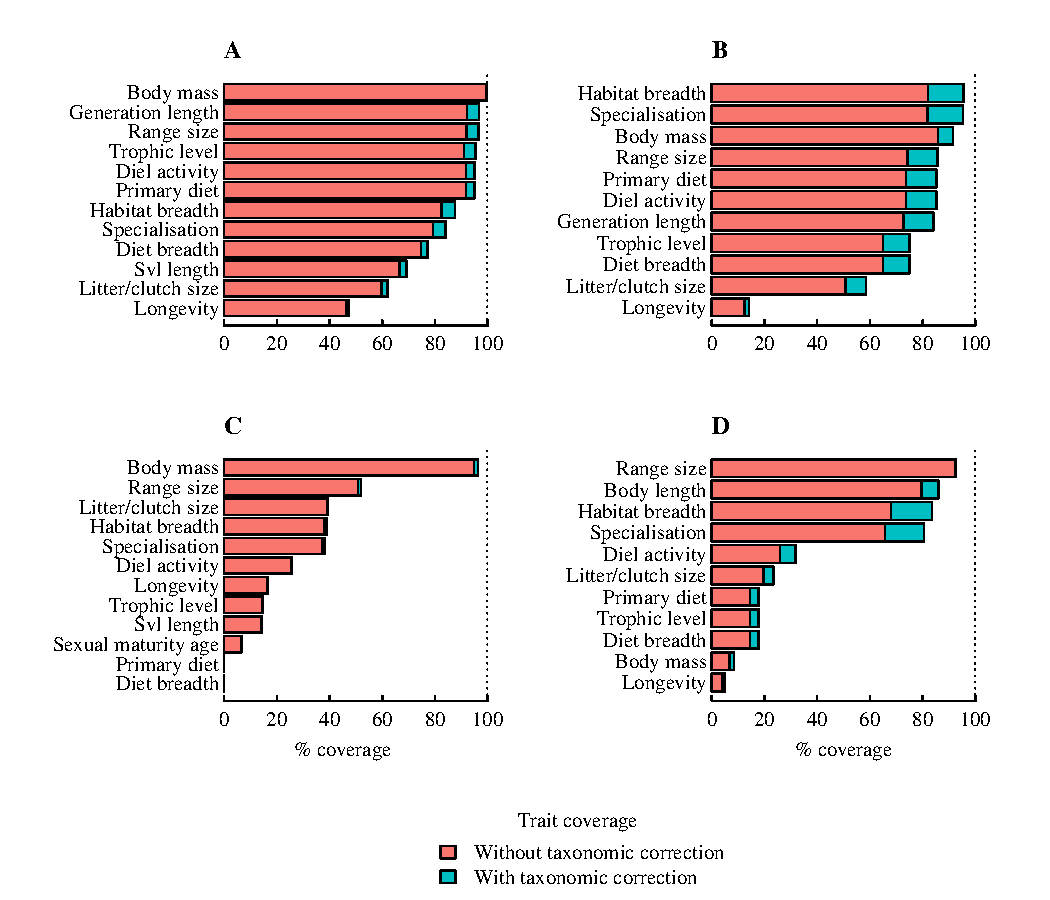
\includegraphics[scale=0.85]{figures/chapter2/Trait_coverage/Predictor_traits/All_species}
\caption[Trait coverage across all species before and after taxonomic correction]{\textbf{Trait coverage across all species before and after taxonomic correction.} Here are shown all targeted traits as well as a few other traits used in imputations, as additional predictors (such as generation length for mammals and birds or body length for amphibians). \textbf{(A)} Mammals (5885 species before correction, 5502 and after correction); \textbf{(B)} birds (13554 species before correction, 11637 after correction); \textbf{(C)} reptiles (10722 species before correction, 10334 after correction) and \textbf{(D)}; coverage across amphibians (8643 species before correction, 6904 after correction). Trait coverage was calculated as the percentage of species for which trait information was available. Correcting for taxonomic synonymy improved coverage in most cases. For mammals and birds, all traits had an initial coverage of more than 50\%, except longevity (but generation lengths were estimated for most species). On the other hand, trait coverage was poor (below 50\%) for about two thirds of collected reptilian and amphibian traits. A clear contrast in trait information appeared between mammals and birds versus amphibians and reptiles, highlighting the existence of important taxonomic biases in data collection.}
\label{traitcov}
\end{figure}

\paragraph{Trait completeness.}
Trait coverage revealed taxonomic biases, with higher resolution of trait information across mammals and birds. Trait completeness reflected similar biases. (Figure \ref{traitcomp}). The median completeness with taxonomic correction was high for mammals and birds (92\% and 82\% respectively) but much lower for reptiles and amphibians (30\% and 36\% respectively). A pairwise Kruskall-Wallis rank sum test rejected the hypothesis that completeness distribution across classes originated from the same distribution (p-values<2$\cdot10^{-16}$ in all cases), showing that class had a significant effect on the availability of trait information. 

\begin{figure}[h!]
\centering
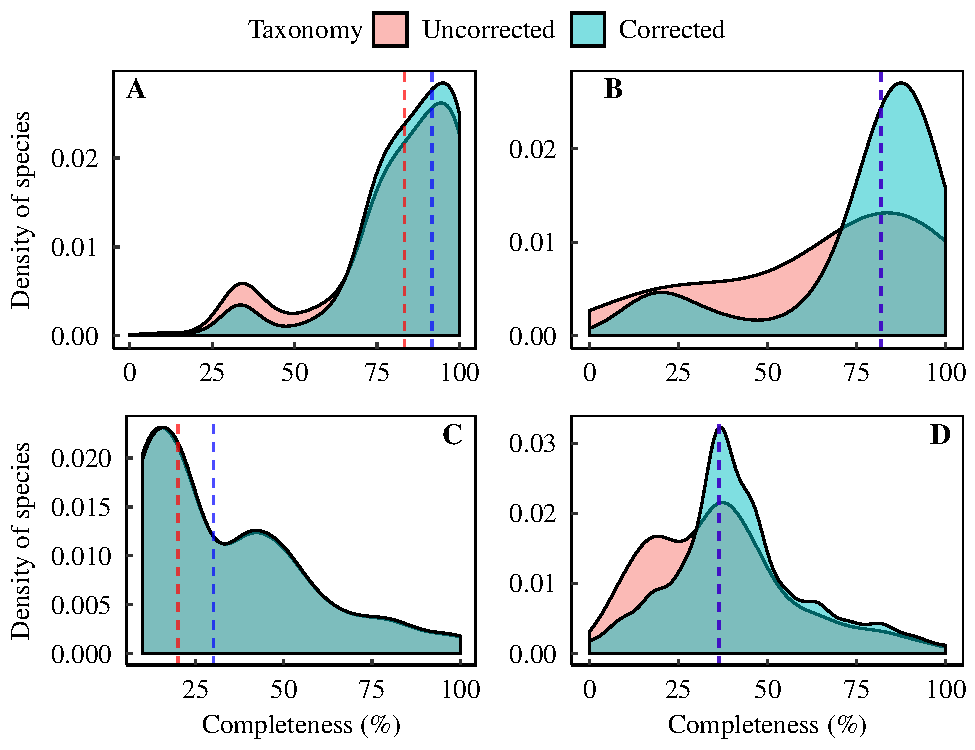
\includegraphics[scale=0.70]{figures/chapter2/Trait_coverage/Missing_values/Traitcompleteness}
\caption[Distribution of completeness of trait information across species]{\textbf{Distribution of completeness of trait information across species.} \textbf{(A)} Mammals; \textbf{(B)} birds; \textbf{(C)} reptiles and \textbf{(D)} amphibians. Completeness was calculated here for the same set of traits shown in Figure \ref{traitcov} (all predictor traits). Correcting for taxonomy affected completeness, significantly shifting the distributions to the right (alternative hypothesis, Wilcoxon rank sum tests: uncorrected medians were lower than corrected medians; mammals: p-value=1.2$\cdot10^{-9}$; birds: p-value<2.2$\cdot10^{-16}$; reptiles: p-value=0.025; amphibians: p-value<2.2$\cdot10^{-16}$). Class had a significant effect on median trait completeness (a pairwise Kruskall-Wallis rank sum test rejected the null hypothesis that completeness distributions across classes originated from the same distribution (p-values<$2\cdot10^{-16}$ in all cases)).}
\label{traitcomp}
\end{figure}

\subsubsection{Non-randomness in trait information availability within classes: patterns of missing trait values with regards to phylogenies}
Beyond cross-class biases in the availability of trait information, within-class patterns of missing values showed that certain families were less sampled than others.

\paragraph{Within-class patterns of trait coverage}

\pagebreak

% Mammals
\begin{figure}[h!]
\centering
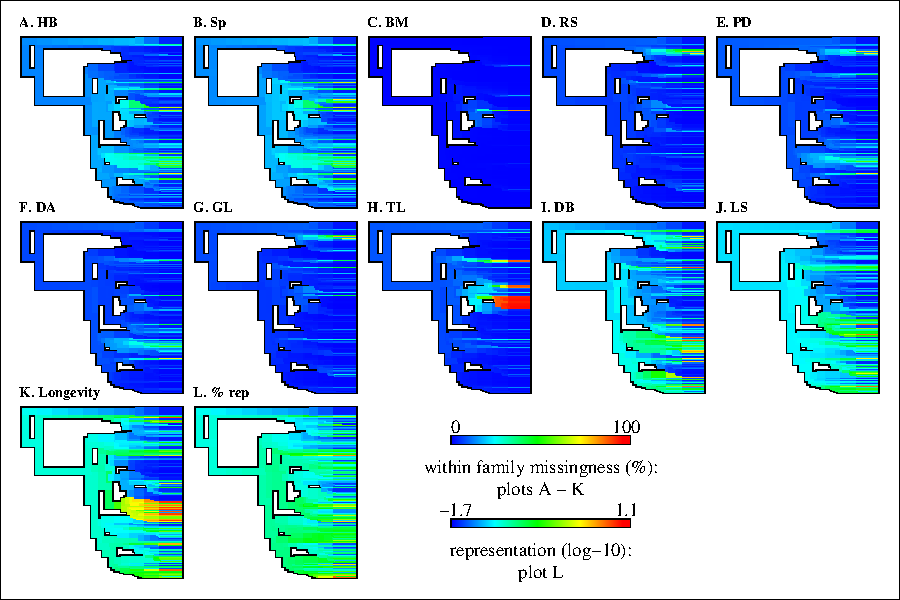
\includegraphics[scale=1]{figures/chapter2/NA_phylo_patterns/Mammals_coverage}
\caption[]{{}}
\label{familycov_mammals}
\end{figure}

% Birds
\begin{figure}[h!]
\centering
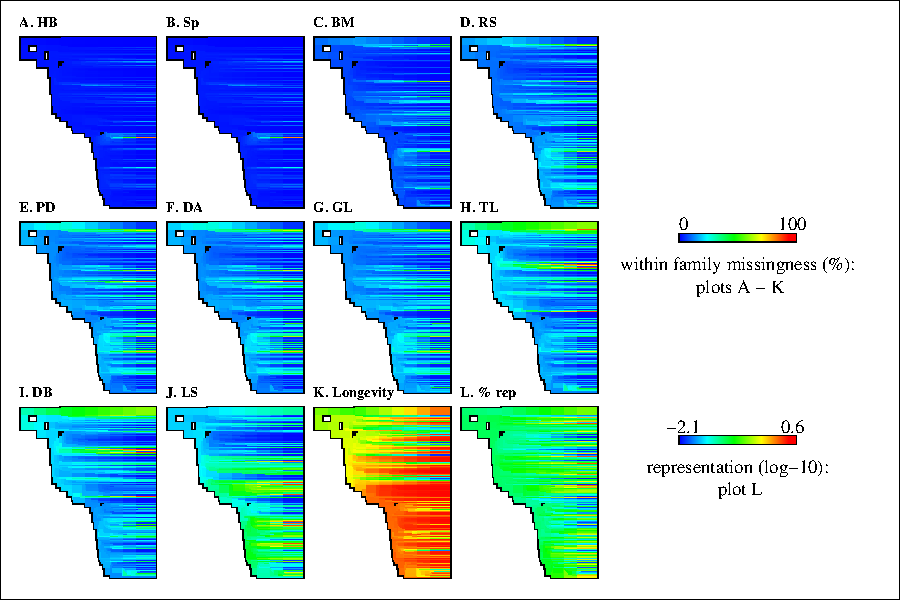
\includegraphics[scale=1]{figures/chapter2/NA_phylo_patterns/Birds_coverage}
\caption[]{{}}
\label{familycov_birds}
\end{figure}

\pagebreak

% Reptiles
\begin{figure}[h!]
\centering
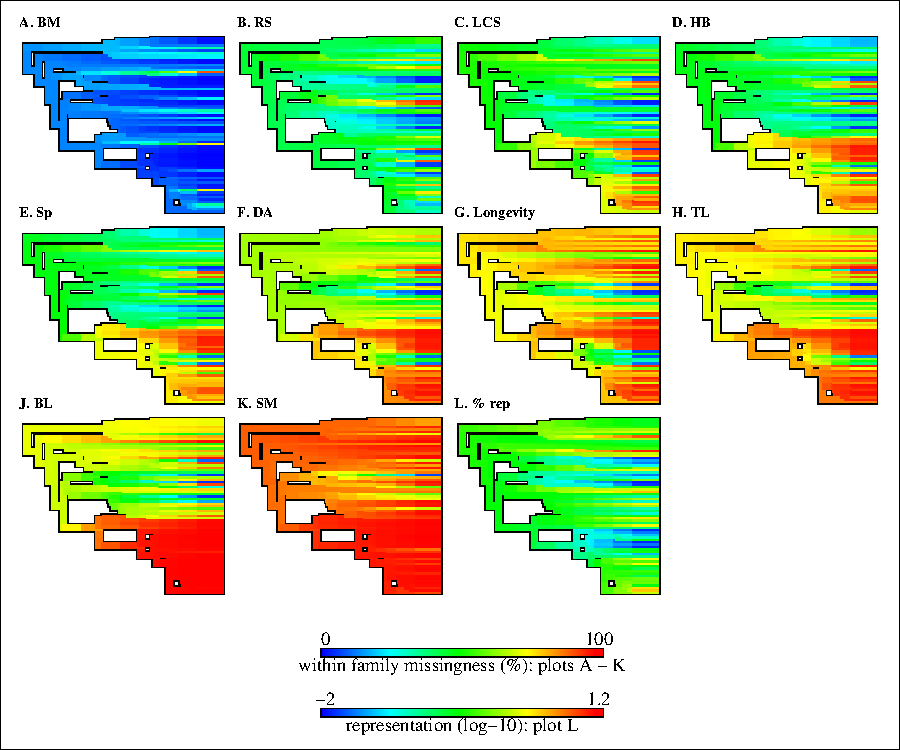
\includegraphics[scale=0.9]{figures/chapter2/NA_phylo_patterns/Reptiles_coverage}
\caption[]{{}}
\label{familycov_reptiles}
\end{figure}

% Amphibians
\begin{figure}[h!]
\centering
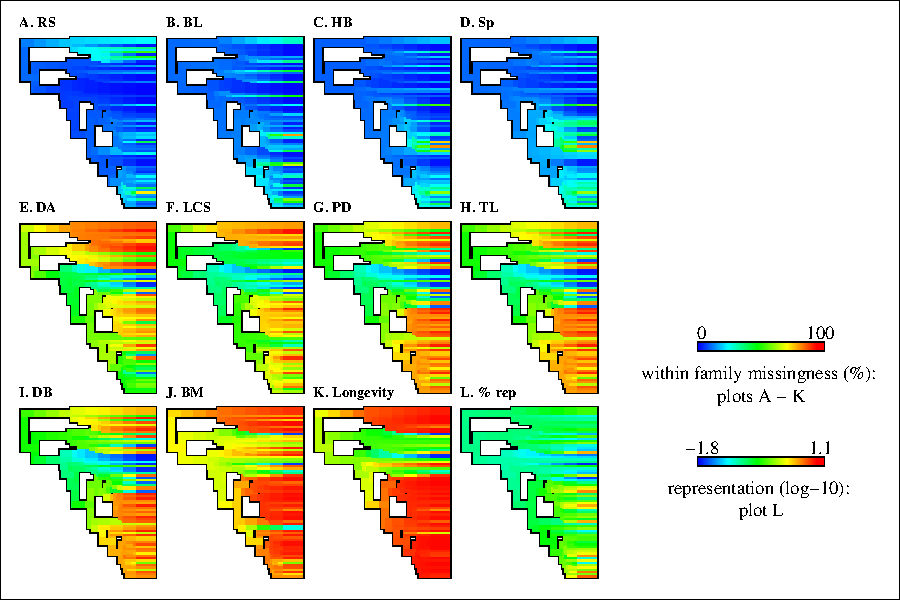
\includegraphics[scale=0.9]{figures/chapter2/NA_phylo_patterns/Amphibians_coverage}
\caption[]{{}}
\label{familycov_amphibians}
\end{figure}


\pagebreak

\paragraph{Within-class patterns of trait completeness}


\begin{figure}[h!]
\centering
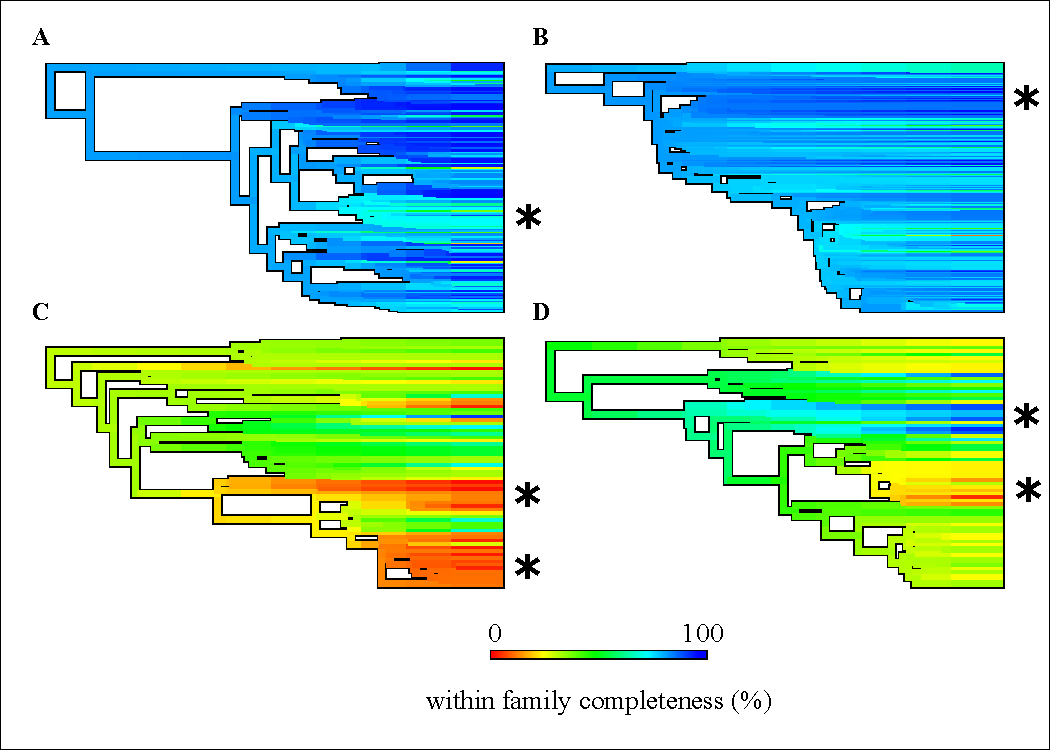
\includegraphics[scale=0.75]{figures/chapter2/NA_phylo_patterns/Completeness_all}
\caption[Median completeness across families]{\textbf{Median completeness across families.} Tips labels are not shown here for better visualisation of the results; the same figures with tip labels are provided in the SI (zooming into the figure is necessary for mammals and birds); tip label information includes order and family. \textbf{(A)} Mammalian family tree; \textbf{(B)} avian family tree; \textbf{(C)} reptilian family tree and \textbf{(D)} amphibian family tree. Median trait completeness was calculated within families and colour-coded  against tree branches.}
\label{classcomp}
\end{figure}

\subsection{Imputation performance and robustness}

\subsubsection{Out-of-bag imputation errors}

\begin{figure}[h!]
\centering
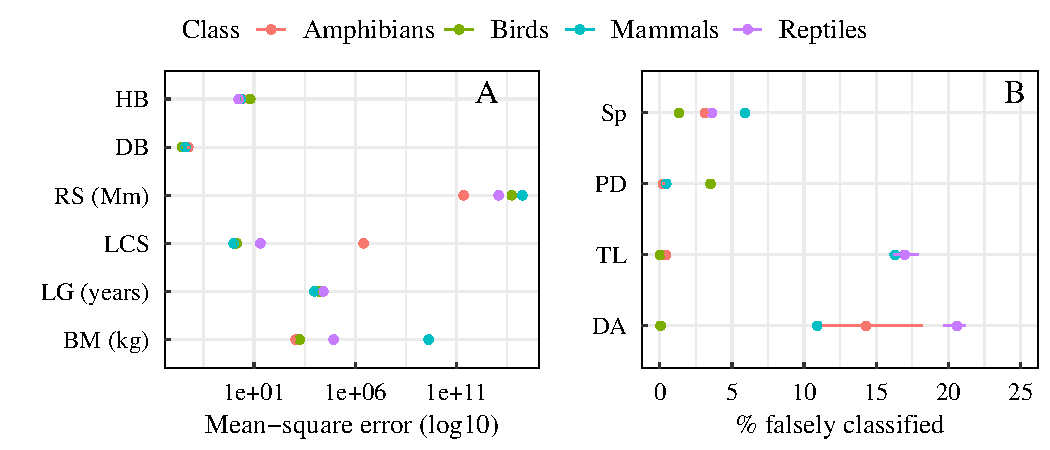
\includegraphics[scale=0.75]{figures/chapter2/Imputation_errors/MSE_PFC}
\caption[missForest mean-square errors and proportion of falsely classified values]{\textbf{missForest mean-square errors and proportion of falsely classified values.} \textbf{(A)} Mean-square errors for continuous traits. \textbf{(B)} Proportion of falsely classified values.}
\label{plotPFC}
\end{figure}

\subsubsection{Congruence of imputed values among 8 imputed datasets}

\begin{figure}[h!]
\centering
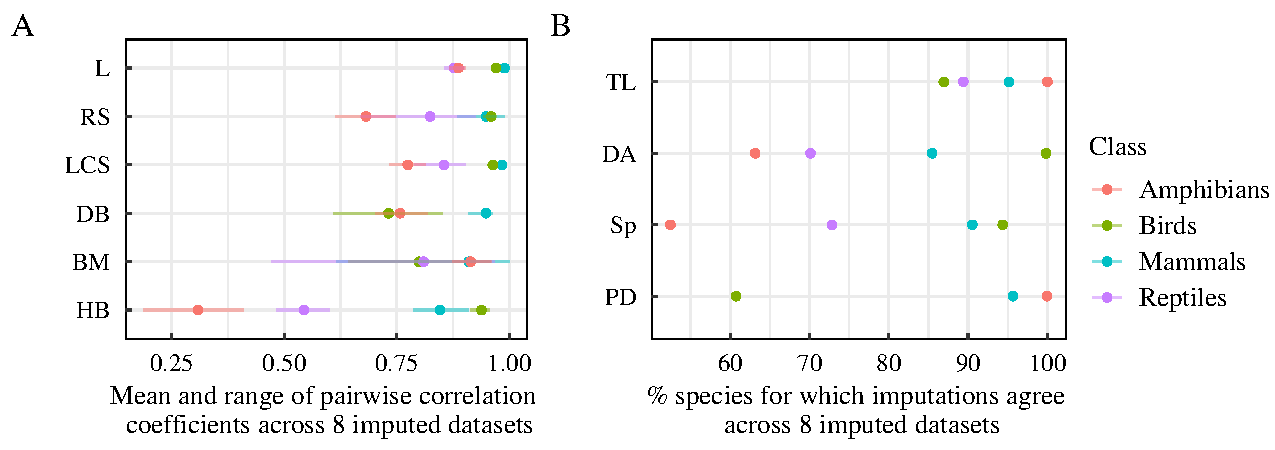
\includegraphics[scale=0.75]{figures/chapter2/Congruence_imputations/Summary}
\caption[]{{}}
\label{plotPFC}
\end{figure}

\subsubsection{Comparison with another collected and imputed datasets for mammals and birds}

\pagebreak
\section{Discussion}
\begin{itemize}
\item Taxonomic challenges
\item Manipulation of the phylogenies
Adding species randomly => justified if traits have a strong phylogenetic signal even with the uncorrected phylogeny. Then adding species makes sense (because strong phylogenetic signal, "trade-off" between the quality of the imputations versus the quality of the phylogenies)
\item Biases in availability of trait information across classes, Raunkier shortfall
\item Imputation robustness 
\end{itemize}
% Finally, I discuss the weaknesses of the methodology
% Impossibility to get intra-specific variation.

Completeness is likely to have an important effect on trait imputations, as it is a reflection of how many predictors have an estimate for a species.

\chapter{Global land-use change promotes the functional homogenisation of local  vertebrate communities}
\section{Introduction}
%% Chapter 3: functional diversity analyses
%Dormann 2012 Collinearity: a review of methods to deal with it and a simulation study evaluating their performance
% Mouillot et al 2014 
\section{Methods}

\subsection{Data sources and trait selection}

\subsubsection{The PREDICTS database: using a `space for time' substitution to assess the impacts of land-use change on local vertebrate communities.}
The impacts of land-use change on the functional diversity of vertebrate communities was assessed using a `space for time' substitution. A longitudinal approach would require data on the evolution of local community composition as the landscape changes from pristine to disturbed, with experimental designs such as `before-after-control-impact' (REF). Nevertheless, such data is difficult to obtain at large scales for diverse taxa and for multiple types of environmental change. With the space for time substitution, a spatial gradient is used as a proxy for temporal dynamics. This approach facilitates meta-analytic studies, as data on the community composition of local assemblages in various land-uses is both easier to collect and more abundant. 

Such data was compiled in the PREDICTS database (ref). This database is, to my knowledge, the most comprehensive global collection of studies that sampled biodiversity across diverse land-uses. In all studies, species abundance (in most cases) or occurrence was recorded across a variety of sites, each characterised by a land-use. Land-use was divided into six categories: primary vegetation, secondary vegetation, plantation forest, cropland, pasture and urban. Secondary vegetation was further divided in three categories (mature, intermediate and young) according to the stage of recovery of the vegetation. %This global database as such allows to conduct meta-analytic studies of the impact of land-use change on terrestrial communities, using a space for time substitution.

I sub-setted the PREDICTS database to retrieve all the sites where vertebrate species were sampled. I selected studies for which the same set of species was consistently sampled across sites, and for which more than one species was considered. Overall, 180 studies were selected (total of 6758 sites). Of these, abundance data was available for 132 studies, and occurrence data for the remaining 48 studies. Figure \ref{PREDICTS_maps} shows the location of all the sites that were considered.

\begin{figure}[h!]
\centering
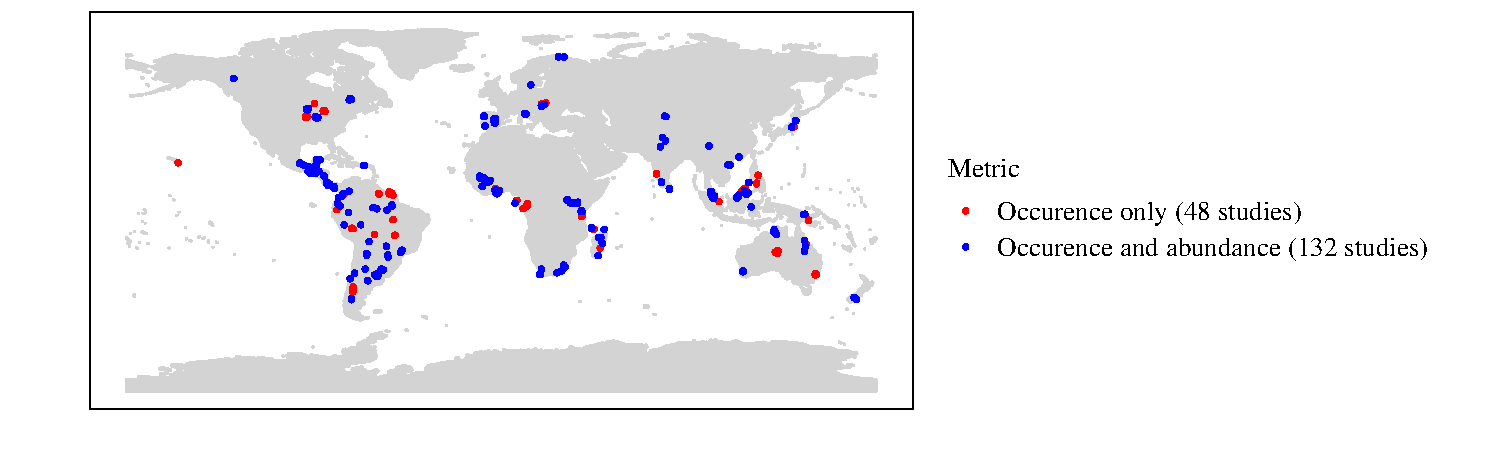
\includegraphics[scale=0.75]{figures/chapter3/Sites}
\caption[Location of selected PREDICTS sites]{\textbf{Location of selected PREDICTS sites.} 180 studies containing occurrence or abundance data for terrestrial vertebrates were selected in the PREDICTS database. Of these, 132 studies provided species relative abundance (corresponding sites are shown in blue on the map). An additional 48 studies only recorded species presence--absence (corresponding sites shown in red).}
\label{PREDICTS_maps}
\end{figure}

As the PREDICTS database was built by collating data from independent studies, its design was imbalanced by construction. As such, nearly half of the selected studies only sampled birds, and nearly 80\% of the studies considered one class only (Table \ref{class_compo}). About 17\% of the studies sampled species from different classes. 

\begin{table}[!htbp] 
\renewcommand{\baselinestretch}{1}
\renewcommand{\arraystretch}{1.2}
\begin{center}\fontsize{9}{11}\selectfont
  \caption[Vertebrate classes considered in selected studies]{\textbf{Vertebrate classes considered in selected studies.} As the PREDICTS database consists of a collation of independent studies...} 
  \label{class_compo} 
\begin{tabular}{@{\extracolsep{1pt}} lcc} 
\\[-1ex]\hline 
\hline \\[-1ex] 
\textbf{Class} & \textbf{Number of studies} & \textbf{\% studies} \\ 
\hline \\[-1ex] 
Birds & $87$ & $48.3$ \\ 
Mammals & $37$ & $20.6$ \\ 
Amphibians & $18$ & $10$ \\ 
Amphibians, Reptiles & $10$ & $5.6$ \\ 
Birds, Mammals & $9$ & $5$ \\ 
Reptiles & $8$ & $4.4$ \\ 
Amphibians, Mammals, Reptiles & $5$ & $2.8$ \\ 
Amphibians, Birds, Mammals, Reptiles & $2$ & $1.1$ \\ 
Birds, Mammals, Reptiles & $2$ & $1.1$ \\ 
Mammals, Reptiles & $2$ & $1.1$ \\ 
\hline \\[-1.8ex] 
\end{tabular} 
\end{center}
\end{table} 

Similarly, the number of sites sampled in each land-use category differed across studies. Table \ref{sample_size_LU} shows the sample size (number of sites) for each land-use category (based on all 180 studies). 

\begin{table}[!htbp]
\renewcommand{\baselinestretch}{1}
\renewcommand{\arraystretch}{1.2}
\begin{center}\fontsize{9}{11}\selectfont
  \caption[Sample size for each land-use category]{\textbf{Sample size for each land-use category.} The number of sites in each land-use is reported here across 180 selected studies.} 
  \label{sample_size_LU} 
\begin{tabular}{@{\extracolsep{5pt}} lcc} 
\\[-1.8ex]\hline 
\hline \\[-1.8ex] 
\textbf{Land-use} & \textbf{Number of sites} & \textbf{\% sites} \\ 
\hline \\[-1.8ex] 
Primary vegetation & $2,569$ & $38.0$ \\ 
Plantation forest & $1,151$ & $17.0$ \\ 
Cropland & $888$ & $13.1$ \\ 
Pasture & $808$ & $12.0$ \\ 
Young secondary vegetation & $501$ & $7.4$ \\ 
Intermediate secondary vegetation & $350$ & $5.2$ \\ 
Urban & $292$ & $4.3$ \\ 
Mature secondary vegetation & $199$ & $2.9$ \\ 
\hline \\[-1.8ex] 
\end{tabular} 
\end{center}
\end{table} 


\paragraph{Trait selection for the calculation of functional indices.}
In Chapter 3, I collected and imputed the values of ten traits across terrestrial vertebrates. Trait data was used in the current Chapter to calculate functional diversity indices. A crucial step was to select the traits to include in the calculations. Indeed, functional diversity indices can be sensitive to the number of traits (Mouillot et al 2014). On the one hand, not including enough traits may lead to missing important areas in the multidimensional trait space. On the other hand, when there is multicollinearity among the traits, functional indices may be inflated. Multicollinearity can create a form of redundancy in the multidimensional trait space, problematic for the calculation of the indices. Assessing whether traits were linearly related to each other was as such a necessary step. 

I randomly selected one imputed trait dataset among the eight imputed datasets (see Chapter 1). To improve normality, a log-10 transformation was applied to all continuous traits (except habitat breadth, which was square-rooted). Trait values were also centred and scaled to zero-mean and unit-variance across the four vertebrate classes. All traits were subsequently considered, except those relating to species diet (primary diet and diet breadth), as these were unavailable for reptiles. As such,the traits taken into consideration were: body mass; longevity; litter/clutch size; habitat breadth; habitat specialisation; diel activity; trophic level.

\begin{comment}
\subparagraph{Dimensionality reduction}

%To first assess if collinearity could be a problem, I used a clustering approach for mixed-type data (factor analysis of mixed type data, or FAMD, ref) to represent the contribution of each variables to principal components. The graph shows that body mass - longevity might e correlated and that BM-LCS could be negatively correlated.


\begin{figure}[h!]
\centering
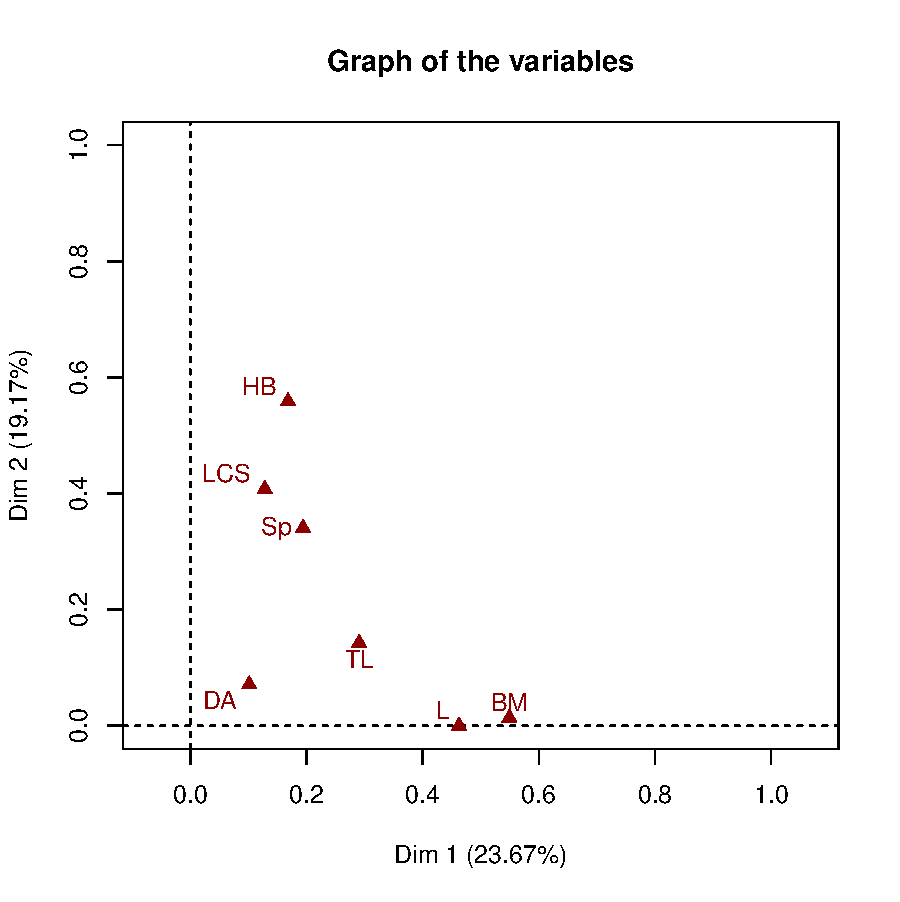
\includegraphics[scale=0.75]{figures/chapter3/Graph_traits_variables}
\caption[]{\textbf{}}
\label{}
\end{figure}

\begin{figure}[h!]
\centering
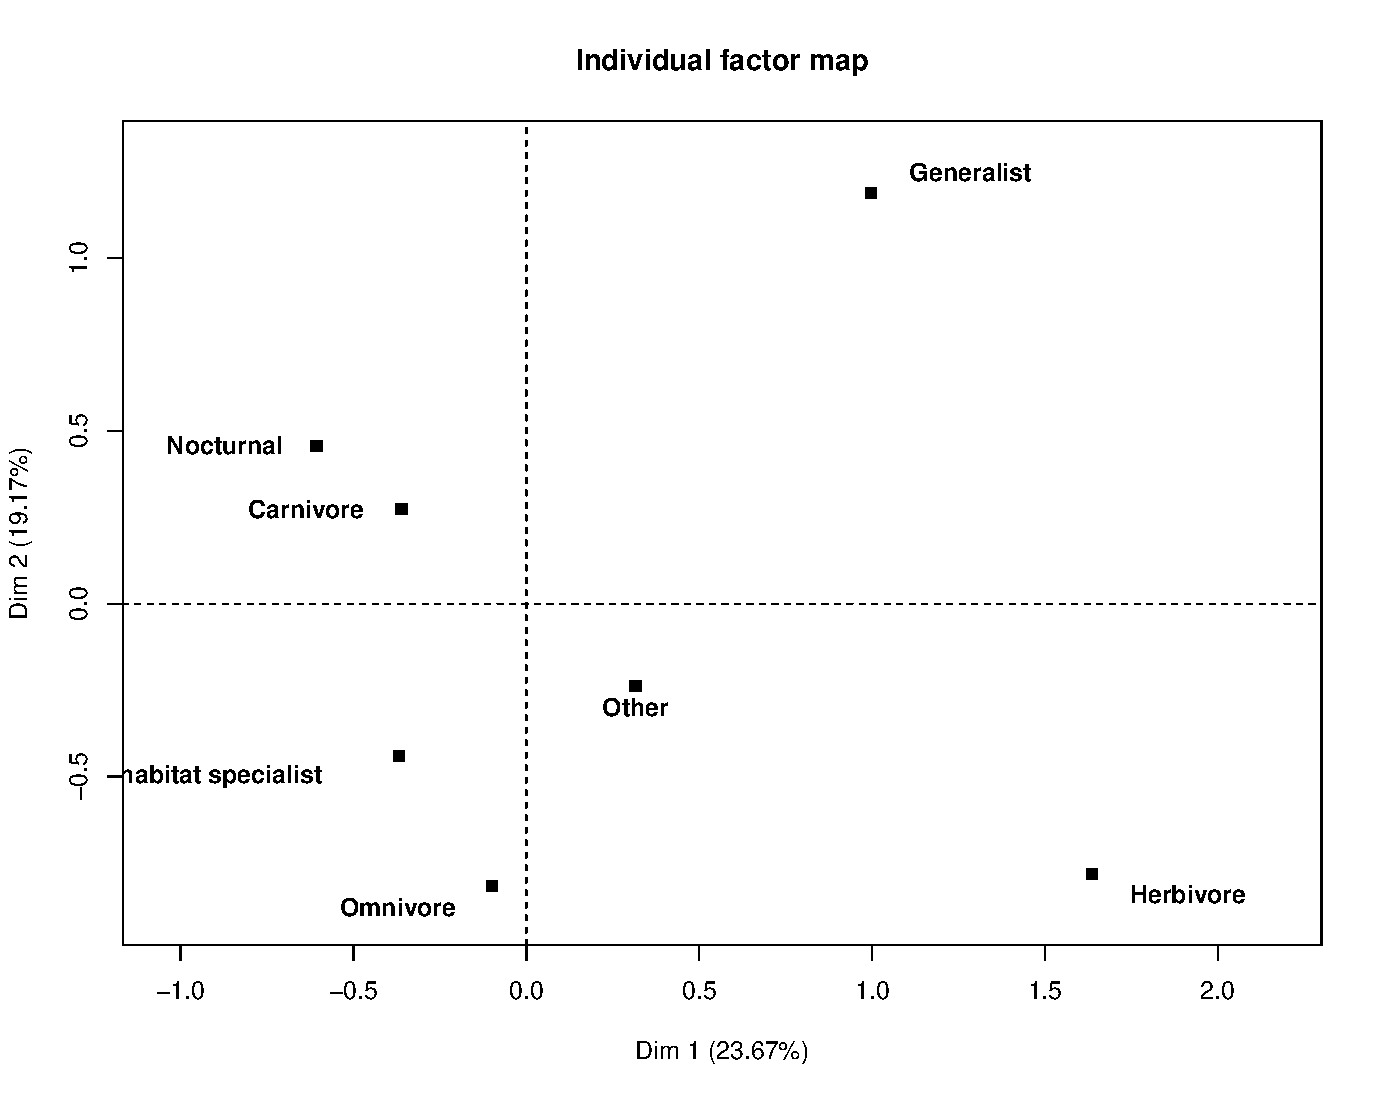
\includegraphics[scale=0.75]{figures/chapter3/Individual_factor_map}
\caption[]{\textbf{}}
\label{}
\end{figure}

\begin{figure}[h!]
\centering
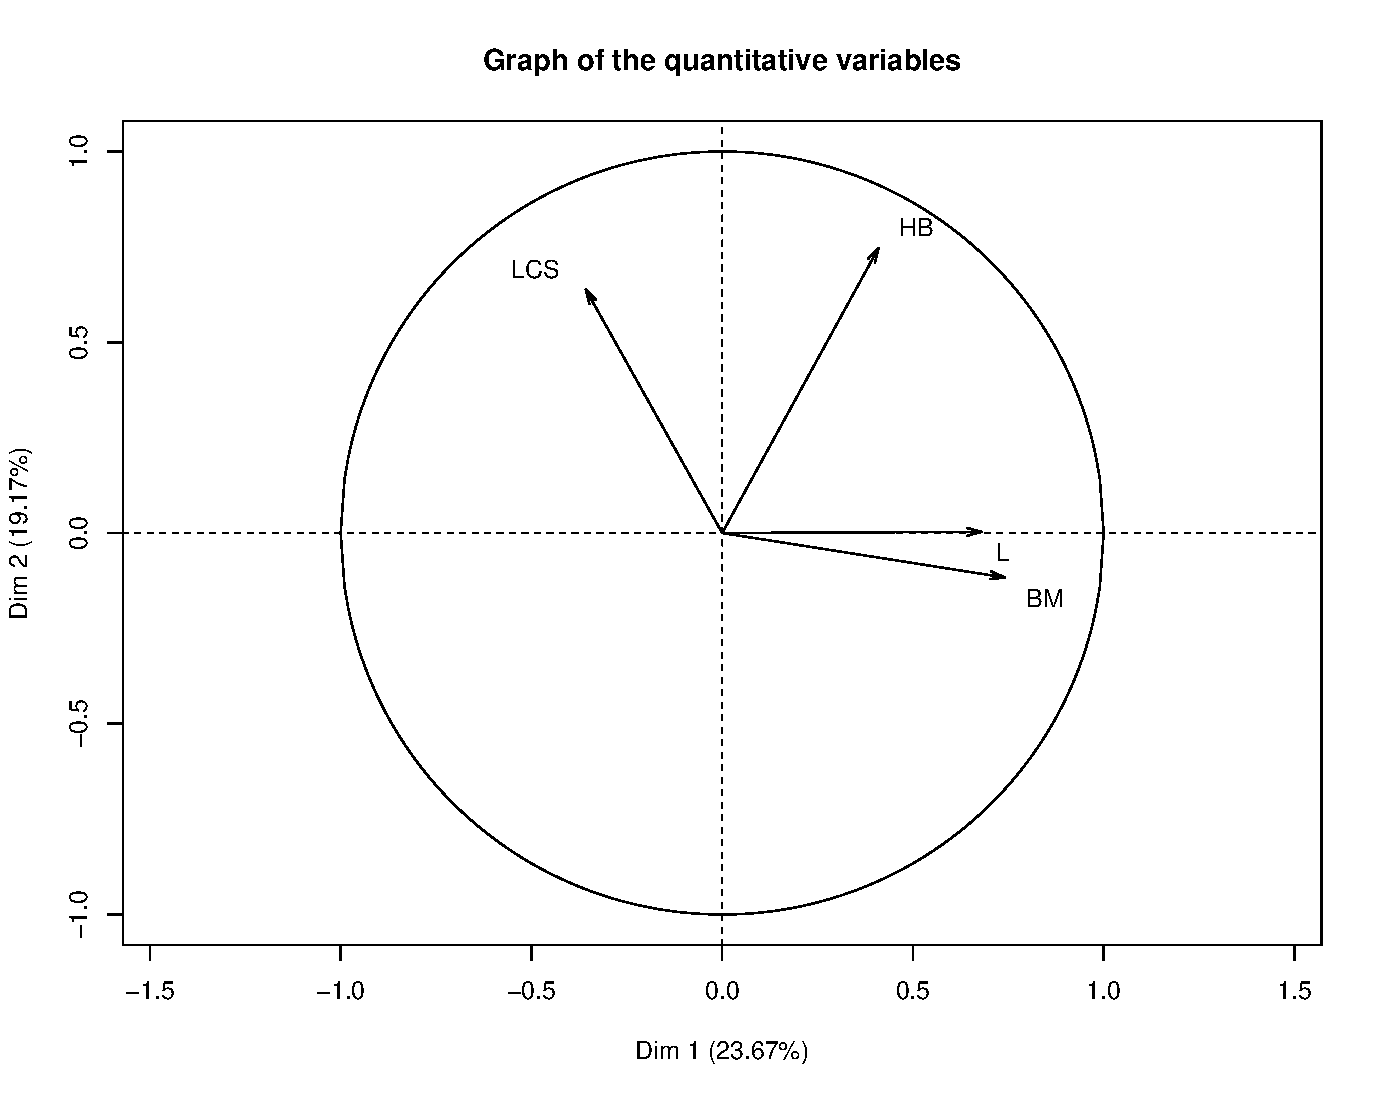
\includegraphics[scale=0.75]{figures/chapter3/Quantitative_variables}
\caption[]{\textbf{}}
\label{}
\end{figure}
\end{comment}

\subparagraph{Assessing the degree of multicollinearity across traits.}
To first assess whether multicollinearity could be a problem, I estimated Pearson's pairwise correlation coefficients among continuous traits, as high correlation coefficients can be an indicator of collinearity. A threshold of 0.7 is usually used for detecting potential collinearity (Dormann 2012). The determinant of the correlation matrix can also be assessed, with values close to 0 indicating high degrees of multicollinearity (Dormann 2012).

Table \ref{corcont} shows the pairwise correlation coefficients among continuous traits. Body mass and longevity were the two variables that had the highest correlation coefficient (0.51). The determinant of the correlation matrix was 0.67, thus indicating that the degree of multicollinearity was likely to be low among continuous traits. 

\begin{table}[!htbp] \centering 
\renewcommand{\baselinestretch}{1}
\renewcommand{\arraystretch}{1.2}
\begin{center}\fontsize{9}{11}\selectfont
  \caption{} 
  \label{corcont} 
\begin{tabular}{@{\extracolsep{5pt}} lcccc} 
\\[-1.8ex]\hline 
\hline \\[-1.8ex] 
 & Body mass & Longevity & Litter/clutch size & Habitat breadth \\ 
\hline \\[-1.8ex] 
Body mass & $1$ & $$ & $$ & $$ \\ 
Longevity & $0.509$ & $1$ & $$ & $$ \\ 
Litter/clutch size & $$-$0.146$ & $$-$0.083$ & $1$ & $$ \\ 
Habitat breadth & $0.167$ & $0.134$ & $0.194$ & $1$ \\ 
\hline \\[-1.8ex] 
\end{tabular} 
\end{center}
\end{table}

Nevertheless, the previous diagnostics did not take into consideration categorical traits. Potential associations between categorical and continuous traits, or among categorical traits, also needed to be assessed. To that end, I used generalised variance inflation factors (GVIF) or variance inflation factors (VIF), as developed by Fox and Monette (1992), to detect multicollinearity across all traits. Given a regression model, variance inflation factors quantify the overestimation in the variance of estimated regression coefficients due to multicollinearity among the predictors. A VIF or GVIF value of 5 or 10 is commonly used as a threshold to select out collinear predictors (Dormann 2012). I used the function stepwise.vif of the package Rnalytica (ref), in which a normally-distributed dummy variable was used as a dependent variable in a linear regression model where all traits were used as predictors. The VIF or GVIF of each predictor was then assessed.  Multicollinearity across predictors was not detected to be problematically high, as all predictors had a VIF or GVIF value below 2 (Table \ref{GVIF}). As such, all the traits figuring in Table \ref{GVIF} were included in the calculations of functional indices. 

% https://www.rdocumentation.org/packages/pedometrics/versions/0.6-6/topics/stepVIF
%% Table GVIF values among traits
\begin{table}[!h]
\renewcommand{\baselinestretch}{1}
\renewcommand{\arraystretch}{1.2}
\begin{center}\fontsize{9}{11}\selectfont
  \caption[Variance inflation factor of estimated regression coefficient for each trait treated as a predictor in a linear regression model.]{\textbf{Variance inflation factor of estimated regression coefficient for each trait treated as a predictor in a linear regression model.} For categorical traits, the GVIF was calculated rather than the VIF. All traits had a VIF or GVIF below 2: multicollinearity was not problematic among the traits.} 
  \label{GVIF} 
\begin{tabular}{@{\extracolsep{5pt}} lc} 
\\[-1ex]\hline 
%\hline \\[-1.8ex] 
 Predictor & VIF or GVIF \\ 
\hline \\[-1.8ex] 
Diel activity & $1.145$ \\ 
Litter/clutch size & $1.267$ \\ 
Trophic level & $1.288$ \\ 
Specialisation & $1.391$ \\ 
Longevity & $1.441$ \\ 
Habitat breadth & $1.473$ \\ 
Body mass & $1.584$ \\ 
\hline \\[-1.8ex] 
\end{tabular} 
\end{center}
\end{table} 


\subparagraph{Ecological relevance of the traits.} See Introduction to Chapter 3. 
% body mass; longevity; litter/clutch size; trophic level;  habitat breadth; degree of habitat specialisation; and diel activity.

\subsection{Definition and calculation of functional diversity indices}


\subsubsection{Calculation of functional diversity metrics across PREDICTS vertebrate communities}
Functional diversity indices were calculated for each local vertebrate community of the PREDICTS database (in other words, for each PREDICTS site, Figure  \ref{FDcalc_chart} A). All indices were calculated across the 180 studies for which species occurrence was available. In addition, indices which could be abundance-weighted were calculated across the 132 studies which provided species relative abundance. 

Rao's quadratic entropy was calculated using the dbFD package (ref).

\subsection{Assessing the impacts of land-use change on functional diversity indices}

	\subsubsection{Functional indices independent from species richness}

	\subsubsection{Functional indices dependent on species richness}

		\paragraph{How does land-use change impact the species-richness--functional richness relationship?}

		\paragraph{Disentangling the effects of species richness from the effects of land-use on functional diversity indices through simulations: an adequate approach with PREDICTS?}

\subparagraph{Approach.}
Functional diversity metrics, notably those aiming at estimating functional richness, can be correlated with species richness. For such indices, disentangling the effects of species richness from the effects of land-use is vital. Indeed, an observed decrease in the main effect of land-use on a functional richness index correlated with species richness may be driven by changes in species richness alone. Above, I detailed how investigating how land-use change affects the species richness -- functional index relationship allows to overcome the species richness problem. Here, I focus on an alternative approach to disentangle the effects of species richness from the effects of another environmental variable.

This approach is based on the randomisation of the species composition of local assemblages. Given a species richness, randomising community composition \textit{m} times allows to generate null expectations of the values of functional indices. These null expectations can then be compared to the empirical (observed) values. Along a species richness gradient, such an approach allows to understand the impact of the variable of interest independently from the impact of species richness on the calculated metrics. Here, such an approach was not necessary \textit{per se}, as most indices were independent from species richness by construction, and for those that were not, I focused on the relationship between species richness and the index rather than on the mean effect of land-use on the effect. Nevertheless, I implemented a simulation approach aiming at examining whether it would be a suitable method given the PREDICTS database.

Specifically, the community composition in each site was randomised by re-sampling species in the corresponding study's species pool, maintaining the species richness of each site (Figure \ref{FDcalc_chart}). Community composition was randomised 1000 times (for metrics calculated with dbFD) or 10,000 times (for DFR). For each randomised community in each site, the functional diversity indices were calculated. Null expectations of functional diversity indices were then generated for each site by taking the median value obtained across simulations.

Although only DFR was strongly correlated with species richness, I implemented this simulation approach for all functional indices that I considered. My expectations were that:
\begin{itemize}
\item For indices independent from species richness by construction, the mean effect of land-use on simulated indices should be similar. Specifically, the mean effect observed for primary vegetation, the most pristine land-use type in the dataset, should not differ from the mean effect observed in other land-uses (\textit{expectation 1}).
\item For indices that correlate with species richness, the slope of the metric--species richness relationship should be similar across land-uses (\textit{expectation 2}). 
\end{itemize} 


\begin{figure}[h!]
\centering
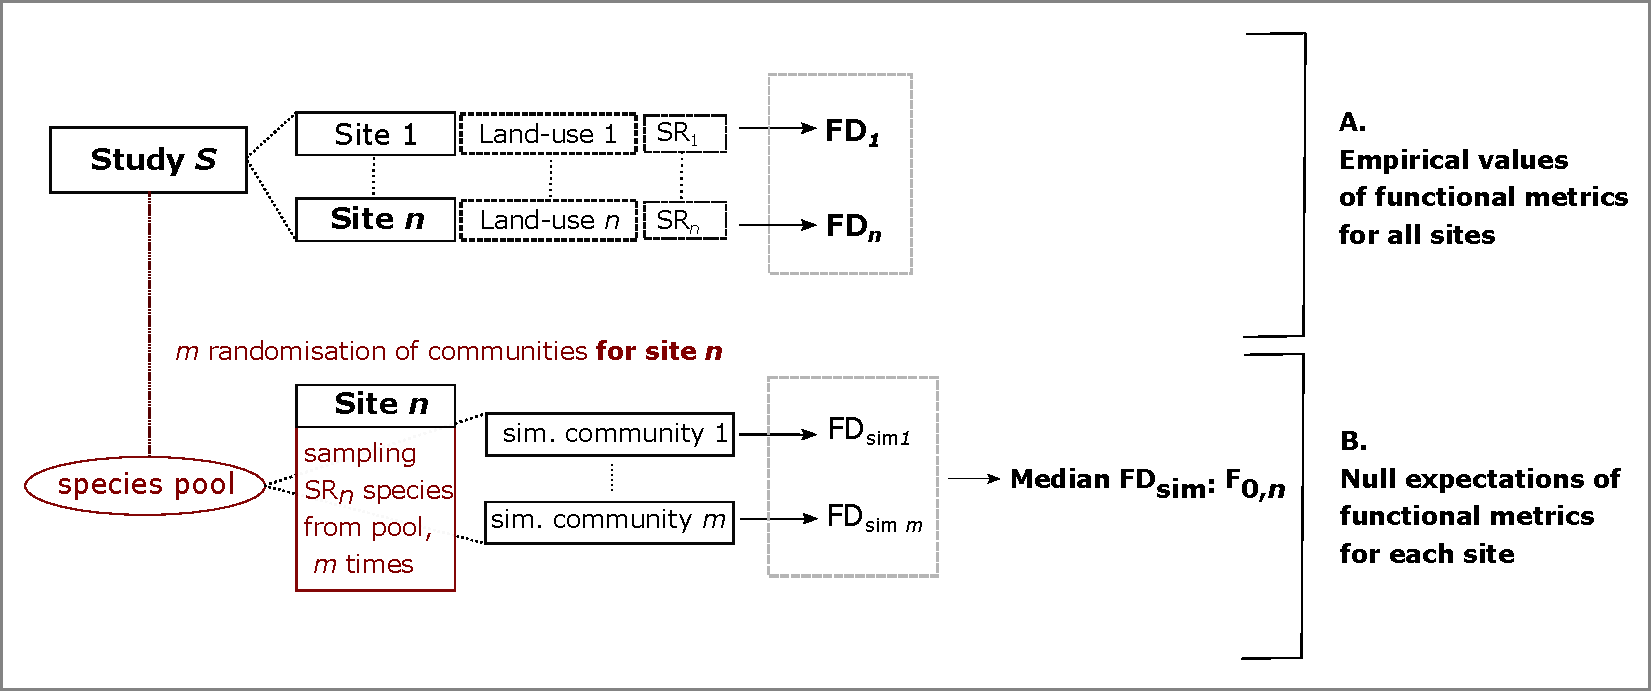
\includegraphics[scale=0.60]{figures/chapter3/chart_FD_calculations}
\caption[Design for calculating functional indices and null expectations for PREDICTS sites]{\textbf{Design for calculating functional indices and null expectations for PREDICTS sites.} \textbf{(A)} Empirical values for the functional diversity indices were obtained for each PREDICTS site, nested within studies. Each site was characterised by its species richness and its land-use. \textbf{(B)} For a given site \textit{n} of richness SR$_{n}$, the community composition was randomised \textit{m} times by drawing SR$_{n}$ species from the study's species pool. Null expectations for the site \textit{n} were then obtained by taking the median value of the indices across simulations.}
\label{FDcalc_chart}
\end{figure}

\subparagraph{Simulation results, and hypotheses as to why simulations may be inadequate.}
Simulation results showed that land-use was having an effect on median simulated values. A decrease in the mean effect was observed for xx and xx, decrease which was significant in some cases, contradicting \textit{expectation 1}. Similarly, a decrease in the slope of the DFR--species richness relationship was observed, contradicting \textit{expectation 2}. I here propose a mechanism that may explain why simulated results differed from my expectations. Simulations were based on the randomisation of the species composition of each site. Species were drawn at random from the species pool, defined as the set of species in each study (equivalent to a `regional' species pool). As such, simulations were sensitive to the composition of the species pool. Nevertheless, the PREDICTS database has an imbalanced design, such that each study do not have sites in all of the land-uses. This may be constricting species pools in some cases. For instance, for a site of land-use `Pasture' belonging to a study where primary vegetation was also sampled, the species pool may be bigger than for a site of land-use `Pasture' where only pasture and plantation forest were sampled. As such, biases in species pool may influence simulation results. Simulation results may capture trends reflecting differences in the size and composition of species pool, which may explain the patterns observed in Figure xx and xx. Figure XX shows Rao's quadratic entropy calculated on the study species pool of each study.

\subparagraph{Simulation approach: conclusion.} The imbalanced design of the PREDICTS database may be causing biases in species pool, which may render simulation approaches difficult to interpret. As such, the simulation approach was not developed further here.

\subsubsection{Dendrogram-based functional richness}
A Gower dissimilarity matrix was first computed from the trait dataset, using the gowdis R function (FD package). This distance matrix contained pairwise distances across all terrestrial vertebrates, based on their trait values. Gower distances allowed to include mixed type variables in the computation. In a second step, this dissimilarity matrix was clustered, to obtain a functional dendrogram, where species presenting similar functional characteristics were closer than more dissimilar species. I used the hclust function, which offers a range of clustering methods. As different clustering methods can have a strong influence on the output dendrogram, I selected the clustering method that best reflected the initial distances in the Gower matrix (correlation coefficient between cophenetic distances obtained from the cluster dendrograms and between the initial dissimilarities in the Gower matrix). The `average' method (unweighted pair group method with arithmetic mean, UPGMA) presented the best correlation coefficient and was as such selected. The resulting cluster dendrogram was a functional dendrogram with 34377 tips, where each tip represented a species. Species position in the tree depended on their functional attributes: species that were functionally more similar were more closely related in the tree.

Finally, functional richness was calculated across all PREDICTS sites. At each site, vertebrate community composition was assessed (species presence/absence), and the functional dendrogram was subsetted according to local community composition. For a site, functional richness was calculated as the sum of the branch length, from root to tip, for the local subset of the functional dendrogram (treedive).


\section{Results}

\subsection{Land-use change constricts the multivariate trait range}
Land-use had a significant effect on volume-based functional richness (Figure \ref{LU_mean_FRic}). For mature and intermediate secondary vegetation, the mean functional richness was similar to that of primary vegetation. For all other more disturbed land-uses, mean functional richness was significantly different from the mean functional richness of primary vegetation, and decreased alongside the land-use gradient. 

\begin{figure}[h!]
\centering
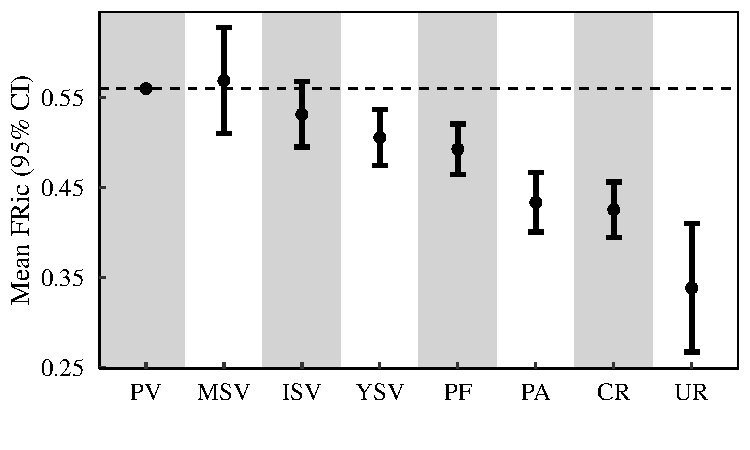
\includegraphics[scale=0.70]{figures/chapter3/FRic/Mean_effect_LU}
\caption[Mean effect of land-use on the volume-based functional richness of vertebrate communities]{\textbf{Mean effect of land-use on the volume-based functional richness of vertebrate communities.} PV: primary vegetation; MSV; mature secondary vegetation; ISV: intermediate secondary vegetation; YSV: young secondary vegetation; PF: plantation forest; CR: cropland; UR: urban. The mean effect corresponds to the estimated fixed effect of a mixed-effect model.}
\label{LU_mean_FRic}
\end{figure}

Because volume-based functional richness is a multivariate analogue of the functional range, Figure \ref{LU_mean_FRic} shows that land-use change significantly impacts the functional composition of local vertebrate communities: species located at the periphery of the functional convex hull are likely to be removed in disturbed land-uses. As such, land-use change significantly impacts the functional composition of local vertebrate communities by constricting the breadth of functions.   

\subsection{Land-use change promotes the functional homogenisation of local vertebrate communities}

\subsubsection{Significant decreases in multivariate trait dispersion}
\begin{figure}[h!]
\centering
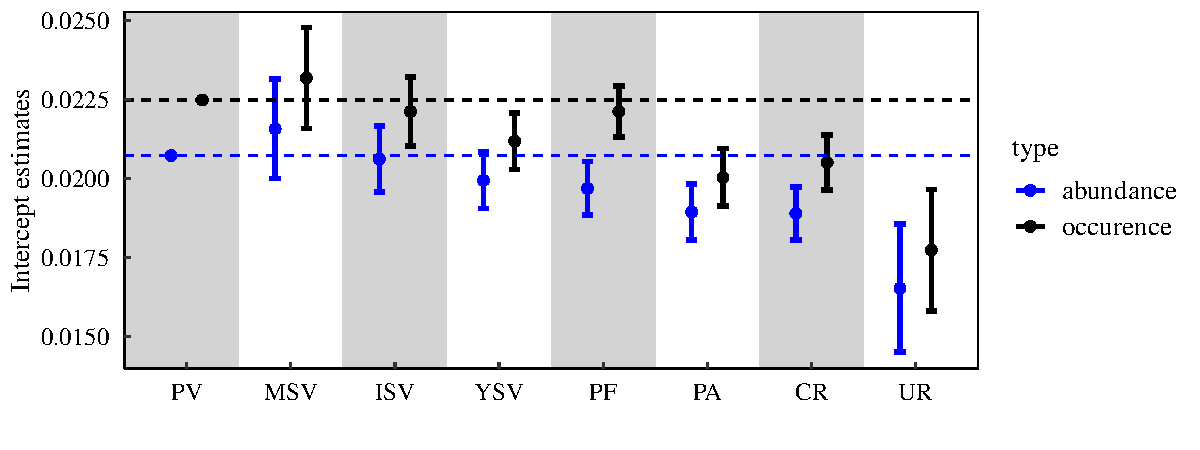
\includegraphics[scale=0.70]{figures/chapter3/RaoQ/Mean_effect_FRaoQ}
\caption[Mean effect of land-use on Rao's quadratic entropy in vertebrate communities]{\textbf{Mean effect of land-use on Rao's quadratic entropy in vertebrate communities.} PV: primary vegetation; MSV; mature secondary vegetation; ISV: intermediate secondary vegetation; YSV: young secondary vegetation; PF: plantation forest; CR: cropland; UR: urban. The mean effect corresponds to the estimated fixed effect of a mixed-effect model.}
\label{LU_mean_FRic}
\end{figure}

%% decreases of functional dissimilarities among species: species become more similar

\subsubsection{Functional redundancy increases}
\begin{figure}[h!]
\centering
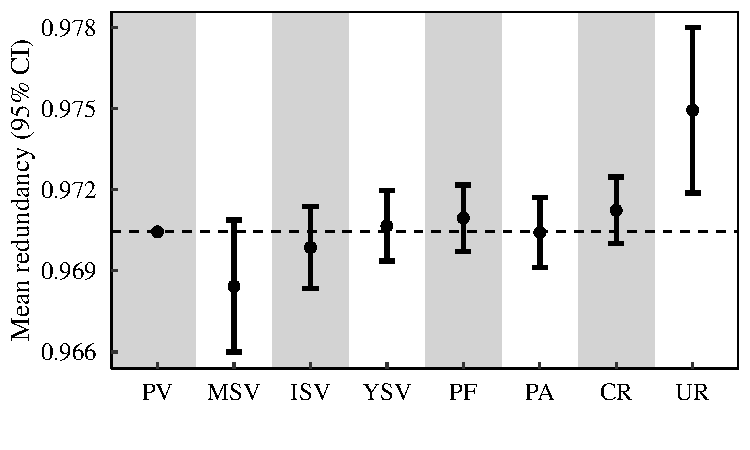
\includegraphics[scale=0.70]{figures/chapter3/FRedundancy/Mean_effect_LU}
\caption[Mean effect of land-use on the functional redundancy of vertebrate communities]{\textbf{Mean effect of land-use on the functional redundancy of vertebrate communities.} PV: primary vegetation; MSV; mature secondary vegetation; ISV: intermediate secondary vegetation; YSV: young secondary vegetation; PF: plantation forest; CR: cropland; UR: urban. The mean effect corresponds to the estimated fixed effect of a mixed-effect model.}
\label{LU_mean_FRic}
\end{figure}



\section{Discussion}
% sensitivity to trait inclusion
% traits that were not considered that could be important, noably home range, dispersal abilities, or volancy -- traits relating to species abilities to move.

\chapter{Future questions}
Here, I outline the future Chapters that I aim to include in my PhD thesis.

\section{Chapter 4: Which traits render species more sensitive to land-use change? }
In Chapter 3, I used functional diversity indices, which enabled to consider multiple traits at the same time to assess the trait composition of ecological communities. Although land-use change was shown to significantly alter the functional diversity of local vertebrate communities, the analyses did not allow to understand which traits conferred species with increased sensitivity to land-use change. Here, I propose to investigate whether species traits render them more sensitive to land-use change. This question has, to my knowledge, never been tackled at global scales comparatively across all four terrestrial vertebrate classes.

Contrary to the previous analyses using functional diversity indices -- where trait composition was summarised into various functional diversity metrics, which were then used as dependent variables in mixed-effect models --, traits will be used as explanatory variables, to explain species occurrence or abundance across land-uses.

Previous work has notably been conducted on tropical forest birds. For instance, \citet{Newbold2013} showed that long-lived, large, non-migratory specialist birds were more sensitive to land-use change than shorter-lived, smaller, migratory generalists. Nevertheless, there is to date no global comparative analyses across the four terrestrial vertebrate classes.

I aim to assess the individual effects of traits on species' sensitivity to land-use using the PREDICTS database. The analyses I propose here are similar to analyses developed in \citet{Newbold2013}. Specifically, I propose to explain species occurrence probability, and given presence, species abundance in each land-use with species traits. The generic mixed-effect models will be written as:  Species occurrence (or abundance)$\sim$Land-use + Traits + Land-use:Traits + RE, where RE is the set of random effects to be included in the model to account for differences in study design across the PREDICTS database (e.g. study identity). Using model selection approaches, I propose to select the best set of traits that explain species presence or species abundances. Then, the analyses of estimated parameters for each trait would indicate the directionality of the effects (and whether effects are consistent across Classes).

\section{Chapter 5: Which traits render species more sensitive to climate change? }
I propose several complementary approaches to investigate which traits are likely to influence species responses to climate change. Using a range of methods would allow to test whether results are robust and consistent. Past studies have used range filling limitations (\cite{Estrada2018, Estrada2016}; see below, \textit{Range filling approach}), historic population trends or recent changes in distributions \citep{Angert2011, Pacifici2017, Mccain2014} or simulation approaches (e.g. comparing empirical estimates with theoretical predictions in \citet{Schloss2012}, or simulating population dynamics to identify the most important predictors of extinction risk in \citet{Pearson2014}), to assess whether certain traits rendered species more sensitive to climate change. Nevertheless, there has been no global study investigating this question across all terrestrial vertebrates.

\subsection{Climatic niche approach}
Here, I propose to use species climatic requirements as a proxy for species sensitivity to future climate change. Species with broader climatic tolerances could be assumed to be less sensitive to future changes.  For a species, climatic tolerances would be measured as the breadth of climatic space covered by the distribution of the species. Climate variables could include temperature, precipitation, water availability for example. Nevertheless, assuming that broader tolerances would indicate lower sensitivity has limitations; species with broader climatic tolerances could be negatively impacted by climate change, if the climate changed beyond the limits of these tolerances, so that much of the climatic space is lost. Similarly, a species with narrow requirements could expand its range if climate change leads to suitable climatic conditions for the species. As such, rather than climatic tolerances, the upper or lower limit of climatic variables could be used. 
For instance, the upper thermal limit of each species could be obtained and compared with projections of future mean temperature in each grid cell. The difference between species upper thermal limit and mean future temperature could be used as a proxy for species exposure to future climate change. 
The aim is then to then assess whether species traits explain species climatic tolerances or exposure, using statistical models (likely, linear models). 

\subsection{Range filling approach}
In this second approach, I propose to investigate whether species traits explain species range filling limitations \citep{Estrada2018}. The range filling of a species is the extent to which the species occupies the area that is climatically suitable. \citet{Estrada2018} suggests that range filling can be used as a proxy for species' abilities to shift their range under climate change. Indeed, several factors could explain that species do not occupy all climatically suitable areas: these non-climatic range filling limitations include, for example, geographical barriers, biotic interactions, edaphic conditions, and life-history traits. 
The degree to which life-history traits explain range limitations could inform on species' ability to track climate change, hence on their sensitivity to the threat. \citet{Estrada2018} conducted an analysis of range filling limitations on European birds, mammals and plants, finding that traits related to establishment and proliferation had a significant effect on mammalian and avian range filling.  To my knowledge, no similar study has been conducted at global scales. Using this approach, I propose to investigate whether vertebrate species traits explain species range filling.

Here, range filling will be assessed by comparing species current ranges to species potential ranges. Species current ranges will be obtained from extent of occurrence maps. Species potential ranges will be determined using species distribution modelling techniques. Potential ranges will be defined as all areas that are climatically suitable for a species. The proportion of the potential range that species actually occupy will then be assessed and will constitute the range filling metric.

\subsection{Population trends approach}
Here, I propose to use historic data on population trends to assess whether both recent climate change and life-history traits explain variation in population trends. The BioTIME dataset \citep{Dornelas2018} contains abundance records for many species, including vertebrates, in the form of time series with a minimal span of one year, allowing for global analyses of historic trends. 

Historic trend data has been used in previous studies to identify traits that correlated with species recent declines due to climate change (for instance at global scales for mammals and birds in \citet{Pacifici2017}; and in mostly North American mammals in \citet{Mccain2014}). Nevertheless, to my knowledge, no study has attempted to consider all terrestrial vertebrates simultaneously. 

One complication when looking at historic climate change is that potential confounding effects could have been shaping species responses (importantly, land-use change). \citet{Spooner2018} analysed global historic avian and mammalian population trends notably using rates of climatic warming, rates of land-use conversion and body mass as explanatory variables. Body mass did not have a significant effect on average rates of population change. Nevertheless, in \citet{Spooner2018}, the effects of land-use and climate change were not studied in isolation. 

I propose to select populations known to have been affected by climate change only. To isolate such populations, I propose to identify areas where primary vegetation is the predominant land-cover (so that it is safe to assume that land-use change has not been not a driver of population change in these areas). For these populations, I propose to investigate whether rates of population change are explained by traits using linear models.

\section{Chapter 6: Projecting species responses to future climate and land-use change: functional diversity under future climate and land-uses} 
Results from Chapter 4 and 5 will allow to assess whether similar traits are likely to put species at greater risk from both land-use and climate change, or whether response traits to land-use and to climate change do not overlap.  Assessing whether the same set of traits is likely to render species more sensitive to both pressures is important to forecast possible interactive effects. 

Here, I propose to use the previous results to build models aiming at projecting species responses to both land-use and climate change given different scenarios. Projections of species occurrence for a scenario of future climate and land-use change will allow several further analyses.

For example, I propose to compare the current functional diversity of vertebrate assemblages to the future functional diversity based on projections. \citet{BarbetMassin2015} conducted such an analysis on birds, with climate change as the pressure being exerted on communities. Nevertheless, to my knowledge, there has been no study looking at the future functional diversity of mammalian and herptilian assemblages, or all vertebrate classes together. 

Both current and future community composition will be assessed using a spatial approach where the intersection between future species ranges will determine assemblage composition in each grid cell. The difference in functional diversity between current and future projections ($\Delta$FD) will then be assessed. 

I will then determine whether future land-use and climate change is likely to have profound impacts on the functional diversity of local vertebrate assemblages by looking at the strength and directionality of $\Delta$FD.  I will assess whether effects are uniform across space and whether certain areas stand out as being particularly sensitive to future climate and land-use change. 


\section{Chapter 7: Will land-use and climate change disrupt important ecosystem functions sustained by terrestrial vertebrates?}
The aim of this part will be to assess whether land-use and climate change are likely to disrupt important ecosystem functions sustained by terrestrial vertebrates. Functional diversity indices calculated in the previous Chapters are unlikely to correlate with specific ecosystem functions, and as such should not be used as proxies for ecosystem functioning. Current knowledge of how land-use and climate change is likely to impact ecosystem processes sustained by vertebrates remains limited at global scales.

I propose to identify vertebrate species that contribute to important ecosystem functions, such as pollination, seed dispersal or nutrient cycling (for instance, scavenging species). Specifically, whether a species belongs to a functional group will be inferred from the species diet. For instance, pollinators will be identified as having nectar and/or flowers as major food items in their diet. Such identification would rely on the trait database compiled in Chapter 2. As reptilian diet is still lacking, reptiles in each functional group could be identified using literature searches. Overall, all identifications could be validated by literature searches, aiming to identify studies that have confirmed experimentally that a given species belongs to a given functional group. Then, I propose to investigate the questions exposed below.

\paragraph{How does land-use change currently affect species in each functional group?}
Here, I propose to investigate whether land-use change adversely impacts the functions sustained by vertebrate species. Species occurrence or abundance in each functional group will be used as a proxy reflecting the maintenance of the associated ecosystem process.

As such, I propose to use the PREDICTS database to investigate whether and how land-use change affects species occurrence or abundance, comparatively across functional groups. To that end, I will build mixed-effect models to explain species occurrence or abundance with land-use, within each functional group. The generic model would be written as: Occurrence (or abundance)$\sim$LU+RE. I will assess whether, on average, certain functional groups are more affected by land-use change than others. The maintenance or endangerment of ecosystem processes sustained by species in each group under land-use change will be inferred from these results.
 
\paragraph{Are all species equally sensitive to land-use and climate change within functional groups?}
Here, I will assess whether species in each functional group are likely to be disproportionally sensitive to land-use or climate change. To that end, I propose to assess the trait composition of each functional group. Using previous results (Chapters 4 and 5), I will assess whether species within each functional group are likely to be equally sensitive to land-use or climate change, or whether there are important variations in species sensitivity to land-use and climate change within each functional group. This question is important to tackle to determine whether certain species could compensate for the loss of other species within each functional group, by performing the same functions at higher rates. 

\paragraph{How will future climate and land-use change impact species in each functional group?}	
Here, I aim to build predictive models of how species in each group will respond to future land-use and climate change, using results from previous Chapters. The likelihood of maintenance or endangerment of ecosystem processes sustained by each functional group will be inferred from future projections. 

\section{Proposed planning}


\begin{landscape}
\begin{figure}[h!]
\centering
\includegraphics[scale=0.9]{figures/chapter4/Ganttchart}
\end{figure}\end{landscape}

\newpage
\addcontentsline{toc}{chapter}{Conclusion}
\chapter*{Conclusion}
I hope to enhance the trait dataset I compiled this last year in the future months of my PhD, notably by adding important traits such as species dispersal ability, volancy, and ability to thermo-regulate. The compilation of diet information for reptiles would also be an important improvement. The analyses of functional diversity indices (as conducted in Chapter 3) could then be conducted again using a broader set of traits. Enhancing the dataset would be beneficial for all further analyses proposed in Chapter 4. Eventually, I hope the trait dataset could be useful to other researchers.
\vskip 0.5cm

In addition to the work presented here, I have followed the trainings and workshops listed below:
\begin{itemize}
\item Introduction to Doctoral Skills Development and the UCL Research Student Log (October 2018); 
\item Arena One Gateway Workshop (mandatory training to teach at UCL) (November 2018); 
\item  Workshop at London Institute of Zoology on the future of biodiversity modelling (November 2018);
\item Management Skills for Researchers (March 2019); 
\item Sweet Dreams; Cultivating Strategies for a Restful Sleep (April 2019); 
\item Nature Research Author Workshop (May 2019);
\item CBER Journal club (throughout the whole year).
\end{itemize}






\clearpage
\chapter*{Bibliography}
\renewcommand{\baselinestretch}{1}
\printbibliography[heading=none]


\end{document}